% Because the content of the project is mainly in Spanish I don't see any reason to not make the comments in Spanish too, from now on, all comments will likely be in Spanish

\documentclass[12pt]{article}

\usepackage[utf8]{inputenc}

\pagenumbering{arabic}

\usepackage[hyphens]{url}

\usepackage[spanish,es-tabla]{babel}
\usepackage[colorlinks, bookmarksopen, linkcolor=red ,citecolor=blue, urlcolor=blue]{hyperref}

% bonito
\usepackage{fancyhdr}
\pagestyle{fancy}

% para pruebas
\usepackage{lipsum}
\usepackage{blindtext}

\usepackage{graphicx}
\graphicspath{ {./gfx/} }

% despues de hyperref para que que funcione correctamente
\usepackage[acronym]{glossaries}
\makeglossaries
\renewcommand*{\glstextformat}[1]{\textcolor{black}{#1}}

\usepackage{float}

% para tener profundidad 4 en las secciones y en la tabla de contenidos
\setcounter{secnumdepth}{4}
\setcounter{tocdepth}{4}
%\chapter - 0
%\section - 1
%\subsection - 2
%\subsubsection - 3
%\paragraph - 4
%\subparagraph - 5

\usepackage{subfigure}

\usepackage{multicol}
\setlength{\columnsep}{1cm}
\usepackage{multirow}

\usepackage{tabularx}

\usepackage{listings}
\usepackage{xcolor}
\definecolor{codegreen}{rgb}{0,0.6,0}
\definecolor{codegray}{rgb}{0.5,0.5,0.5}
\definecolor{codepurple}{rgb}{0.58,0,0.82}
\definecolor{backcolour}{rgb}{0.95,0.95,0.92}
\lstnewenvironment{csharp}[2][]{%
  \lstset{%
    title = #2,
    #1,
    language=[Sharp]C,
    backgroundcolor=\color{backcolour},   
    commentstyle=\color{codegreen},
    keywordstyle=\color{magenta},
    numberstyle=\tiny\color{codegray},
    stringstyle=\color{codepurple},
    basicstyle=\ttfamily\footnotesize,
    breakatwhitespace=false,         
    breaklines=true,                 
    captionpos=b,                    
    keepspaces=true,                 
    numbers=left,                    
    numbersep=5pt,                  
    showspaces=false,                
    showstringspaces=false,
    showtabs=false,                  
    tabsize=2
  }%
}{}

\usepackage{pdfpages}

\usepackage{verbatim}

\usepackage{datetime}

% comandos
\newcommand\tab[1][1cm]{\hspace*{#1}}
\newcommand{\quotes}[1]{``#1''}

\begin{document}

\begin{center}

    
\includegraphics[width=0.8\textwidth]{logo_ulpgc_version_horizontal_positiva_de_uso_cotidiano_a_2_tintas.png}
    
    
\includegraphics[height=0.2\textheight]{gfx/eii-logo-texto.png}\\[0.4cm]


    {\Large Universidad de Las Palmas de Gran Canaria}\\[0.2cm]
    {\Large Grado en Ingeniería Informática}\\[0.2cm]
    {\Large Trabajo Fin de Título}\\[0.2cm]

    {
      \LARGE\bfseries Implementación de InputStick en la app Android de Bitwarden para escritura automática de contraseñas \\[0.2cm]
    }
    {\large Autor}\\[0.1cm]
    \textsc{\large Pablo Ortigosa Quevedo}\\[0.4cm]
    {\large Tutor}\\[0.1cm]
    \textsc{\large Antonio Ándres Ócon Carreras}\\[0.4cm]
    Junio, 2023
\end{center}

\newpage

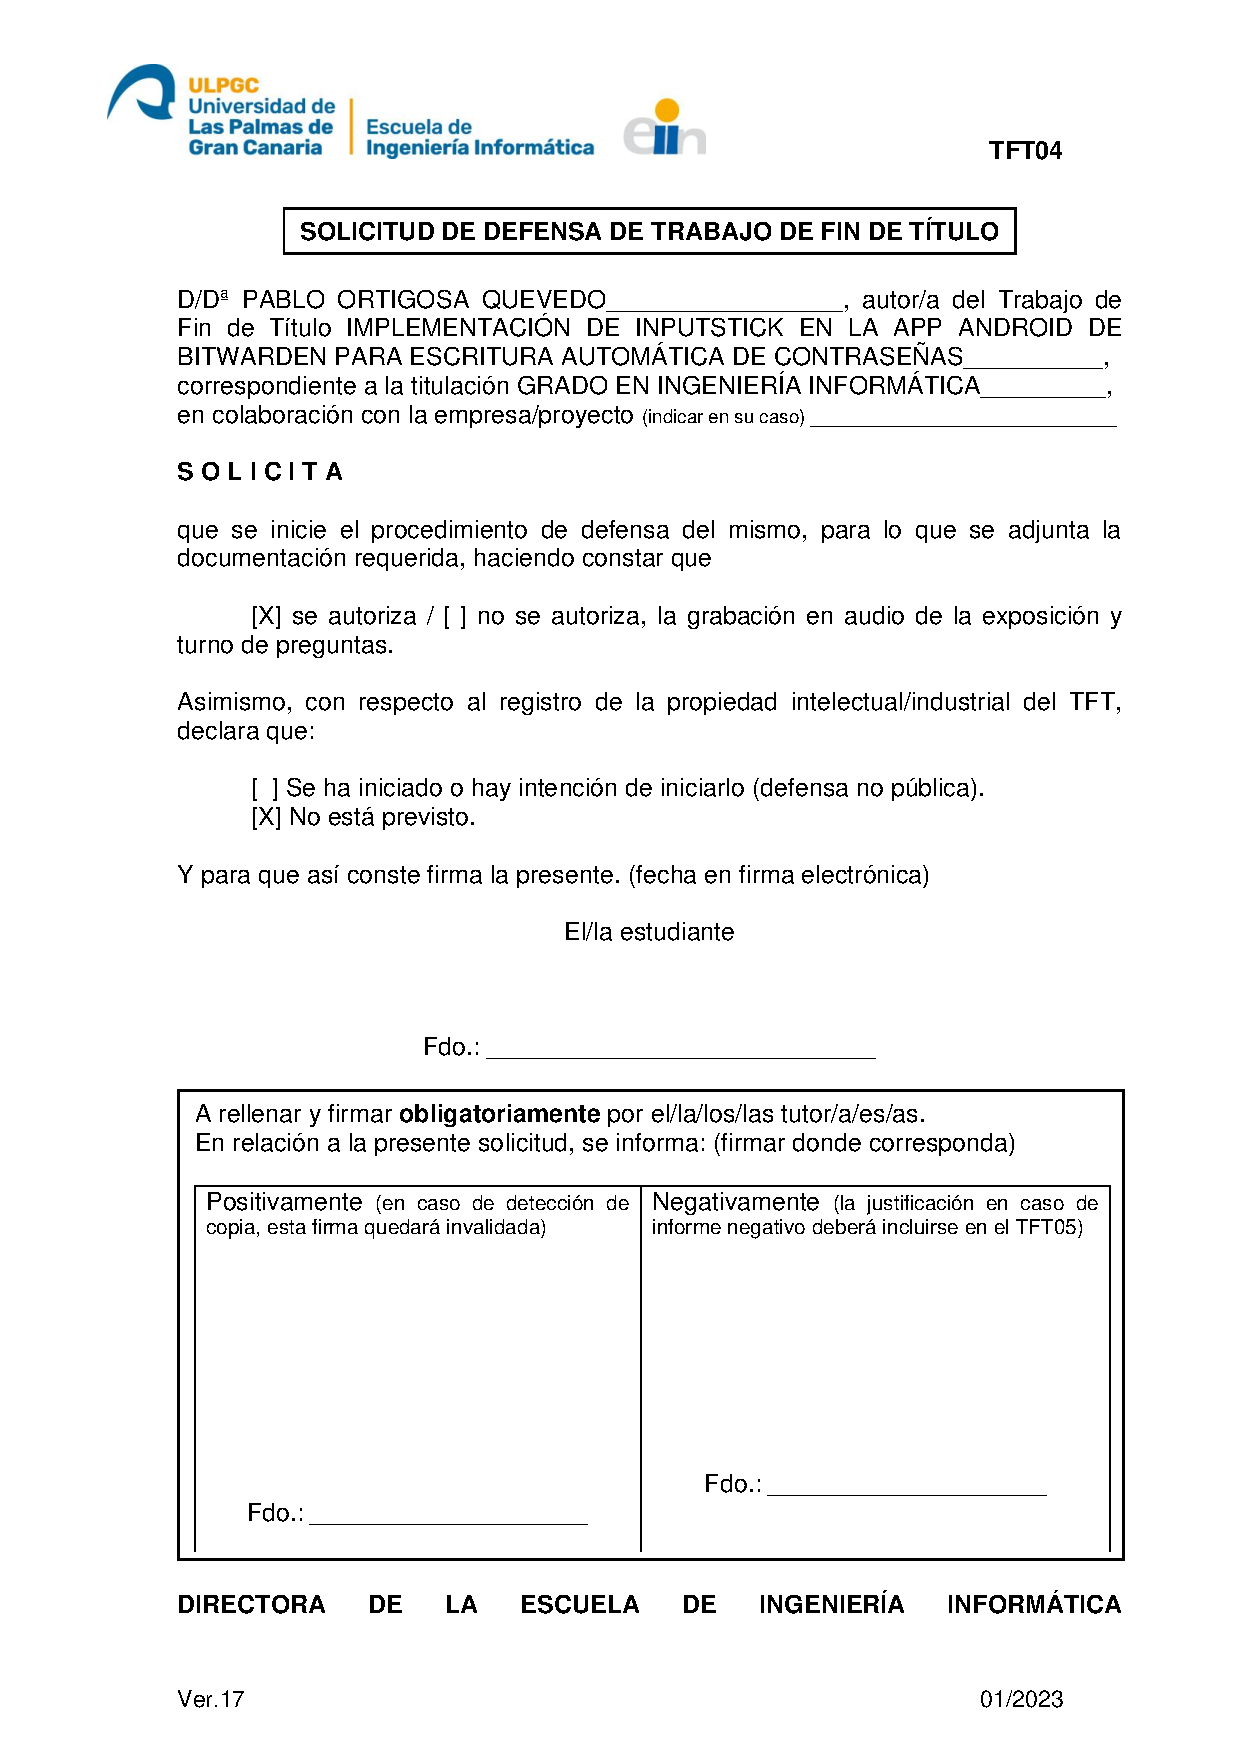
\includepdf[pages={1}]{TFT04-v17.pdf}
\newpage

{
\glsresetall
{\huge{\textbf{Resumen}}}
\newline\newline
{\indent\large{Modificación de la aplicación Android de Bitwarden, un administrador de contraseñas en la nube, con el fin de añadir soporte para InputStick, un receptor \gls{usb} Bluetooth que simula un teclado \gls{hid}. Con esto se lograría escribir una contraseña en dispositivos compatibles con el estándar \gls{hid} mediante \gls{usb}, que no tienen ningún cliente de Bitwarden instalado y sin necesidad de usar el cliente web. Por tanto se lograría evitar escribir la clave maestra en un dispositivo en el que no se confía y así sólo poner en riesgo la clave que se necesite usar en el momento. }
\glsresetall
\newpage
{\huge{\textbf{Abstract}}}
\newline\newline
{\indent\large{Modificacion of the Android aplication of Bitwarden, a password manager on the cloud, with the objective of adding support for InputStick, a Bluetooth \gls{usb} receiver that simulates a \gls{hid} keyboard. This would make possible to type a password in devices compatible with the \gls{hid} standard through \gls{usb}, that do not have a Bitwarden client installed and without the need to use the web-interface client. This way we would accomplish the feat of avoiding writing the master password in an untrusted device so the only password that could be compromised would be the one needed at the moment.}}
}
\newpage

% glosario
\newglossaryentry{vault}{name={bóveda},description={\textit{vault}. Donde Bitwarden almacena los credenciales de las distintas cuentas del usuario. Adicionalmente en este informe se usa indistintamente para referirse también a una cuenta de Bitwarden}}
\newglossaryentry{cuenta}{name=cuenta,description={Cuando se hable de cuenta se habla de a lo que un \textit{\gls{login}} hace referencia, que principalmente suelen ser cuentas de servicios web. Cuando se refiera a una cuenta de Bitwarden se usará el término \gls{vault}}}
\newglossaryentry{login}{name={elemento de cuenta},description={\textit{Login item}: Par de credenciales Usuario-Clave\cite{item}}}
\newglossaryentry{freemium}{name=\textit{freemium},description={De \textit{free} y \textit{premium}. Que ofrece un servicio gratuito además de una opción de pago}}

% acronimos y siglas
% si provienen del inglés están en cursiva
\newacronym{usb}{USB}{\textit{Universal Serial Bus}}
\newacronym{hid}{HID}{\textit{Human Interface Device}}
\newacronym{api}{API}{\textit{Application Programming Interface}}
\newacronym{vpn}{VPN}{\textit{Virtual Private Network}}
\newacronym{cli}{CLI}{\textit{Command Line Interface}}
\newacronym{aes}{AES}{\textit{Advanced Encryption Standard}}
\newacronym{sha}{SHA}{\textit{Secure Hash Algorithm}}
\newacronym{e2ee}{E2EE}{\textit{End-to-end encryption}}
\newacronym{url}{URL}{\textit{Uniform Resource Locator}}
\newacronym{uri}{URI}{\textit{Uniform Resource Identifier}}
\newacronym{totp}{TOTP}{\textit{Time-based One-time Password}}
\newacronym{2fa}{2FA}{\textit{Two-factor Authentication}}
\newacronym{hmac}{HMAC}{\textit{Hash-based Message Authenthication Code}}
\newacronym{pnp}{PnP}{\textit{Plug and Play}}
\newacronym{ble}{BLE}{\textit{Bluetooth Low Energy}}
\newacronym{bios}{BIOS}{\textit{Basic Input/Output System}}
\newacronym{pbkdf}{PBKDF}{\textit{Password-Based Key Derivation Function}}
\newacronym{srp}{SRP}{\textit{Secure Remote Password}}
\newacronym{qmk}{QMK}{\textit{Quantum Mechanical Keyboard}}
\newacronym{zmk}{ZMK}{\textit{Zephyr Mechanical Keyboard}}
\newacronym{mvvm}{MVVM}{\textit{Model-View-ViewModel}}
\newacronym{mvc}{MVC}{\textit{Model-View-Controller}}
\newacronym{mvp}{MVP}{\textit{Model-View-Presenter}}
\newacronym{jbl}{JBL}{\textit{Java Bindings Library}}
\newacronym{uml}{UML}{\textit{Unified Modeling Language}}
\newacronym{gui}{GUI}{\textit{Graphical User Interface}}
\newacronym{cryptomac}{MAC}{\textit{Message Authentication Code}}
%\newacronym{addressmac}{MAC}{\textit{Media Access Control}}

%-----------------------

{
    \hypersetup{linkcolor=black}
    \tableofcontents
    \newpage

    % figuras
    \listoffigures
    \newpage

    % tablas
    \listoftables
    \newpage
}
% glosario
\printglossary
\newpage

% acrónimos
\setacronymstyle{long-short}
\printglossary[title={Siglas y acrónimos},type=\acronymtype,nonumberlist]
%,title=Abreviaciones, toctitle=Índice de abreviaciones
\newpage

\glsresetall

\section{Conceptos previos}
\subsection{Bitwarden}
Bitwarden es un administrador de contraseñas código abierto en la nube, donde se guardan los credenciales de las distintas \glspl{cuenta} del usuario. Se accede a la base de datos desde los distintos clientes:
\begin{itemize}
    \item Escritorio
    \item Web
    \item Extensión de navegador
    \item \gls{cli}
    \item \textbf{App de Android}
    \item App de iOS
\end{itemize}

\begin{figure}[H]
    \centering
    
\includegraphics[width=\textwidth]{gfx/bitwarden-logo-horizontal.png}
    \caption{Logo de Bitwarden. \href{https://github.com/bitwarden/brand}{Realizado por Bitwarden.}}
    \label{fig:bitlogo-horizontal}
\end{figure}

Una vez en un cliente el usuario puede crear una \gls{vault} donde almacenar los credenciales de inicio de sesión en distintos servicios.
Los clientes de Bitwarden almacenan una caché de la \gls{vault} para así poder acceder a ella incluso cuando no pueden conectarse al servidor \cite{bitcache}.
Todo esto ocurre bajo un método de conocimiento cero \gls{e2ee}, y los credenciales sólo son descifrados en memoria.
Existen distintos tipos de servidores Bitwarden:
\begin{itemize}
    \item Servidor oficial: Servidor de la propia empresa Bitwarden.
    \item Self-host: Alojar una estancia manualmente en un servidor propio.
    \item \textbf{Vaultwarden}: Implementación de la \gls{api} de los servidores de Bitwarden en Rust, \textit{self-host}.
\end{itemize}

\begin{figure}[H]
    \centering
    
\includegraphics[width=\textwidth]{gfx/vaultwarden-logo.png}
    \caption{Logo de Vaultwarden. \href{https://vaultwarden.discourse.group/}{Realizado por Vaultwarden.}}
    \label{fig:vaultlogo}
\end{figure}

Para este proyecto se modificará la app de Android y se usará como servidor una estancia en red local de Vaultwarden.
\subsection{InputStick}
Actualmente existen 2 modelos InputStick: Bluetooth 2.1 y Bluetooth 4.0.\cite{stickversions} :a versión que usamos en este proyecto es la 4.0 ya que es más reciente, por ello siempre que hablemos de InputStick nos estaremos refiriendo a la versión 4.0.

InputStick es un dispositivo \gls{usb} con conexión Bluetooth. Cuando está conectado a un dispositivo mediante el puerto \gls{usb}, InputStick actúa como un periférico \gls{hid}, mientras que a través de la conexión Bluetooth se le indica a InputStick qué hacer, en nuestro caso será simular presionar las teclas de un teclado. \ref{fig:inputstick-diagram} \cite{stickworks}

\begin{figure}[H]
    \centering
    
\includegraphics[width=\textwidth]{gfx/inputstick-logo.png}
    \caption{Logo de InputStick. \href{http://inputstick.com/}{Realizado por InputStick}}
    \label{fig:inputstick-logo}
\end{figure}

\begin{figure}[H]
    \centering
    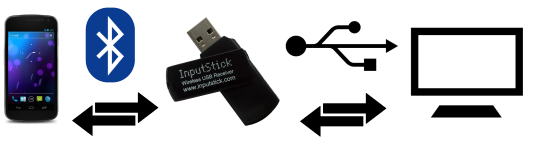
\includegraphics[width=\textwidth]{gfx/inputstick-diagram.png}
    \caption{Diagrama  de conexión InputStick. \href{http://inputstick.com/how-it-works/}{Realizado por InputStick}}
    \label{fig:inputstick-diagram}
\end{figure}
Debido a su capacidad de dispositivo \gls{hid}, InputStick puede hacerse pasar como:
\begin{itemize}
    \item \textbf{Teclado}
    \item Ratón
    \item Controlador de Videojuegos
    \item Botones multimedia
    \item Pantalla táctil
\end{itemize}

Como medida de seguridad InputStick usa conexión Bluetooth cifrada\cite{stickfaq}, además es posible activar el protocolo de cifrado \gls{aes}-128 para enviar datos, y se verificarán usando \gls{hmac}-\gls{sha}256\cite{sticksecurity}. Esta clave se puede configurar de 2 formas, ambas desde la app InputStickUtility:
\begin{itemize}
    \item De forma no segura: La clave se envía a InputStick, por lo que para ello no se puede usar una clave.
    \item De forma segura: Se le solicita a InputStick que genere una clave, InputStick procederá a escribirla en el dispositivo que se encuentre conectado, ahora el usuario la puede copiar a mano, ya que la puede ver en pantalla.
\end{itemize}

InputStick nombra a la frecuencia de reportes de escritura como velocidad, así que usaremos la misma terminología, aunque técnicamente sea incorrecto, como al hablar de la velocidad de la memoria RAM, que en realidad es frecuencia.
\newpage
\section{Prólogo}
\subsection{Motivación}
Tras ver a un compañero introducir su clave maestra de Bitwarden en un dispositivo en el cuál no confiábamos surgió la duda y el problema de cómo evitar esta situación. Tras ello discutimos situaciones similares con sus inconvenientes e investigamos superficialmente sobre el tema, llegando así al \textit{abstract} de este proyecto como una solución a dicho problema. Es por tanto el objetivo de este proyecto investigar la proposición, desarrollarla y valorar la viabilidad, la seguridad y la conveniencia de esta. En resumen la pregunta a resolver es: ¿Cómo podemos introducir los credenciales de un servicio de forma cómoda y segura en la mayoría de dispositivos?
\subsection{Introducción}
En este mundo digital en el que vivimos, parte de los elementos más importantes son los credenciales a las diversas \glspl{cuenta} que pueda tener un usuario. Por ello estos credenciales no deberían repetirse ya que constantemente estos credenciales son expuestos al público tras ataques informáticos\cite{pwnedwebs}, sin embargo somos seres humanos, así que desafortunadamente nuestra memoria nos puede fallar, por lo que es surrealista esperar que un usuario recuerde todos los credenciales de sus diversas \glspl{cuenta}. Por ello es recomendable usar un administrador de contraseñas.

Con una \gls{vault} de Bitwarden este problema se soluciona fácilmente. Sin embargo acceder a una \gls{cuenta} no siempre es tan fácil, en concreto cuando se quiere entrar a una \gls{cuenta} en un dispositivo desconocido. Existen 2 formas de lograrlo:
\begin{itemize}
    \item Introducir los credenciales de la \gls{cuenta}, exponiendo entonces a este dispositivo desconocido la clave maestra de la \gls{vault}
    \item Buscar los credenciales en la \gls{vault} y enviarlos por Bitwarden Send, o escribirlos a mano.
\end{itemize}

En el caso de acceder directamente a la \gls{vault} desde el dispositivo objetivo, existen situaciones específicas en las que es imposible o bien poco seguro:
\begin{itemize}
    \item Cuando la clave es el inicio de sesión del propio dispositivo, la forma de desbloquear el mismo, por tanto, aún no se puede tener acceso a la \gls{vault}.
    \item Cuando el dispositivo no posee conexión a internet, por ejemplo, acceder a una base de datos interna de una empresa \textit{on-site}.
    \item Cuando se pone en duda la seguridad del dispositivo. Aunque, por supuesto con \gls{2fa} activada tendríamos una gran protección ante la posibilidad de que alguien con intenciones maliciosas conozca nuestra clave maestra, pero no por ello deberíamos ir pregonando dicha clave, como hizo el actual multimillonario Gabe Newell en 2011. \cite{gabepass}
    \item Cuando el dispositivo objetivo se encuentra bastante limitado, sin permisos de administrador, sin acceso a navegador y/o sin aplicación nativa de Bitwarden. Por ejemplo una consola de videojuegos o una Smart TV.
\end{itemize}

Por otro lado el servicio Bitwarden Send\cite{sendblog} está planteado para \textbf{enviar} datos, información, \textbf{claves} y archivos \textbf{a otras personas}, pero se sigue pudiendo usar personalmente para enviarse a uno mismo una contraseña, como antaño cuando no era popular el almacenamiento online y uno se enviaba un correo electrónico con un archivo porque se había olvidado el pendrive en casa. Aún así crear un Send es un poco rudimentario, pues requiere muchos pasos y el \gls{url} es bastante largo como para escribirlo a mano. \ref{fig:send-link}
\begin{figure}[H]
    \centering
    
\includegraphics[width=\textwidth]{gfx/send-link.png}
    \caption{Un \gls{url} de Bitwarden Send. \href{https://bitwarden.com/blog/bitwarden-send-how-it-works/}{Realizado por Bitwarden}.}
    \label{fig:send-link}
\end{figure}
Adicionalmente si la estancia de Bitwarden se encuentra en una red local tras una \gls{vpn} o similar en vez de en un dominio público, sólo se podría acceder al enlace si el dispositivo objetivo se encuentra conectado a la misma \gls{vpn}.

Así llegamos a la solución que en este proyecto hemos implementado. Hoy en día, es muy poco probable no llevar un móvil encima, por ello lo cómodo y simple sería que el móvil escribiese por nosotros los credenciales específicos, evitando así exponer la clave maestra. Para llevar a cabo dicha tarea usaremos InputStick como medio de transmisión.
\subsection{Estado del arte}
\subsubsection{Administradores de contraseñas}
\begin{itemize}
    \item 1Password
    \begin{itemize}
        \item En la nube
        \item Propietario
        \item Suscripción de pago
        \item Seguridad: \cite{1passencryption}
        \begin{itemize}
            \item \textit{Zero knowledge encryption}
            \item \gls{pbkdf}2-\gls{hmac}-\gls{sha}256
            \item \gls{srp}
        \end{itemize}
    \end{itemize}

    \item Bitwarden
        \begin{itemize}
            \item En la nube
            \item Open source
            \item Suscripción \gls{freemium} con alternativa \textit{self-host}
            \item Seguridad: \cite{bitencryption}
            \begin{itemize}
                \item \textit{Zero knowledge encryption}
                \item \gls{e2ee} \gls{aes}256
                \item \textit{Salted hashing}
                \item \gls{pbkdf}2 \gls{sha}256
            \end{itemize}
        \end{itemize}

    \item KeePass
    \begin{itemize}
        \item Local
        \item Open source. KeePassXC es una implementación de KeePass en C++.
        \item Gratuito
        \item Seguridad: \cite{keepencription}
        \begin{itemize}
            \item \textit{Zero knowledge encryption}
            \item \gls{aes}256
            \item Chacha20
            \item \gls{sha}256
        \end{itemize}
    \end{itemize}

    \item LastPass
    \begin{itemize}
        \item En la nube
        \item Propietario
        \item \Gls{freemium}
        \item Seguridad: \cite{lastencryption}
        \begin{itemize}
            \item \textit{Zero knowledge encryption}
            \item \gls{aes}256
            \item \textit{Salted hashing}
            \item \gls{pbkdf}2 \gls{sha}256
        \end{itemize}
    \end{itemize}
    \item Authorizer \cite{authorizer}
    \begin{itemize}
        \item Local
        \item Open Source
        \item Gratuito
        \item Seguridad:
        \item Autoescritura:
        \begin{itemize}
            \item Por \gls{usb}. Requiere una modificación del kernel de Android.
            \item Por Bluetooth. El dispositivo objetivo necesita poder establecer una conexión Bluetooth directa.
        \end{itemize}
    \end{itemize}
    
\end{itemize}
\subsubsection{Dispositivos de escritura automática}
\begin{itemize}
    \item Arduino:
    Las placas arduino basadas en procesadores 32u4 o SAMD pueden usarse como dispositivo \gls{hid} \cite{arduinokeyboard}. Con esto resuelto el resto podría hacerse fácilmente, con un módulo de pantalla táctil y ser independiente o bien con un módulo Bluetooth y depender de otro dispositivo. Incluso con otro arduino que actúe como \textit{master} y una conexión \gls{usb} a otro dispositivo este podría dar las órdenes por el puerto serial. Esto de hecho era el primer planteamiento de este proyecto, sin embargo ni hace falta reinventar la rueda, ni parece una alternativa cómoda el llevar una placa encima, comparado con llevar un \quotes{pendrive} (InputStick no es un pendrive pero tiene la misma forma y tamaño) en el llavero.
    \item Firmware:
    Existen diversos lenguajes de firmware para teclados, con ellos se podría resolver la escritura automática:
    \begin{itemize}
        \item \gls{qmk} \cite{qmk}
        \item KMK \cite{kmk}
        \item Vial \cite{vial}
        \item \gls{zmk} \cite{zmk}
        \item VIA \cite{via}
    \end{itemize}
    La mayoría requieren placas basadas en procesadores 32u4 o SAMD, como las placas arduino.
    \item InputStick
    
    \item Raspberry Pi Zero

    \item Android:
    
    \begin{itemize}
        \item Laa. Requiere Bluetooth o wifi. \cite{laa}
        \item Android keyboard gadget. Funciona por \gls{usb}, requiere root ya que modifica el kernel de android. \cite{android-keyboard-gadget}. 
            por usb, requiere root.
        \item BLE HID over GATT Profile for Android. Requiere Bluetooth. \cite{BLE-HID-Peripheral-for-Android}
    \end{itemize}
\end{itemize}
% scrapped, si bien estas opciones existen, distan bastante del trabajo por lo que no se va a comentar nada al respecto
% - RubberDucky BashBunny
% - logitech https://github.com/bilogic/logitech-unifying-device
\newpage

\newpage

\section{Proyecto}
\subsection{Objetivos}
Los objetivos de este proyecto son los siguientes:
\begin{itemize}
    \item Soporte para InputStick en Bitwarden: Se pretende que se puedan escribir los credenciales mediante InputStick a través de Bitwarden de la forma más cómoda posible. Solucionando así el problema de escribir claves complejas en dispositivos que no soportan clientes de administradores de contraseñas. Además debe ser fácil de entender y usar para el usuario menos experimentado y que esta implementación no destaque por encima de ninguna otra funcionalidad de la app, gráfica y programáticamente, que parezca que esta funcionalidad estuvo siempre ahí.
    \item Escribir código en un programa \quotes{grande} y observar los diversos patrones y estilos que se usen en este código profesional. Analizando el mismo y aprendiendo de este.
    \item Escribir código en una aplicación para dispositivos móviles y observar qué hay que tener en cuenta para ello.
\end{itemize}
\subsection{Competencias}
\subsubsection{TFG01}
<<Ejercicio original a realizar individualmente y presentar y defender ante un tribunal
universitario, consistente en un proyecto en el ámbito de las tecnologías específicas de la
Ingeniería en Informática de naturaleza profesional en el que se sinteticen e integren las
competencias adquiridas en las enseñanzas.>>\newline
La realización de este trabajo cuya idea proviene de un problema que se expone en el día a día, buscando extender las funcionalidades de un programa informático \quotes{grande} como es la app de Android de Bitwarden.

\subsubsection{CII08}
<<Capacidad para analizar, diseñar, construir y mantener aplicaciones de forma robusta, segura
y eficiente, eligiendo el paradigma y los lenguajes de programación más adecuados.>>\newline
La modificación de código en una aplicación \quotes{grande} requiere un estudio previo de dicha aplicación para que la modificación sea coherente y consistente.

\subsubsection{CII017}
<<Capacidad para diseñar y evaluar interfaces persona computador que garanticen la
accesibilidad y usabilidad a los sistemas, servicios y aplicaciones informáticas.>>\newline
El estudio y modificación de la \gls{gui} para añadir funcionalidad nueva.

\subsubsection{CII018}
<<Conocimiento de la normativa y la regulación de la informática en los ámbitos nacional,
europeo e internacional.>>\newline
La modificación de código abierto implica el estudio de las licencias a las que está sujeto.

\subsubsection{IS01}
<<Capacidad para desarrollar, mantener y evaluar servicios y sistemas software que
satisfagan todos los requisitos del usuario y se comporten de forma fiable y
eficiente, sean asequibles de desarrollar y mantener y cumplan normas de
calidad, aplicando las teorías, principios, métodos y prácticas de la ingeniería del
software.>>
El estudio de un código en una aplicación \quotes{grande} implica el estudio de patrones de diseño de la ingeniería del software

\subsubsection{TI07}
<<Capacidad para comprender, aplicar y gestionar la garantía y seguridad de los sistemas
informáticos.>>\newline
El estudio de un administrador de contraseñas y la proposición de enviar estas claves de forma segura a InputStick.
\subsection{Análisis}
Parte del análisis, en concreto los patrones de de diseño, se investigó en paralelo que la implementación, cuando algo resultaba no ser como creíamos había que revisar lo comprendido de analizar el código de la aplicación. Por ello esta sección pretende parte el marco teórico del proyecto aprendido de observar el código de Bitwarden. Mientras que más adelante se discutirá la parte práctica. Por tanto el orden aquí expuesto no representa el orden cronológico del proyecto.

\subsubsection{Historias de usuario}
\begin{itemize}
    \item Cernuda es un joven al que le encanta ver a sus creadores de contenido favoritos, como Ibai, AuronPlay o ElRubius. Para verlos usa la plataforma \textit{Twitch}. Cernuda quiere iniciar sesión en su \textit{Smart TV}, pero como usuario de Bitwarden su clave es muy larga y por lo tanto tosca de introducir con el mando a distancia.
    \item Lorca es un fanático de los videojuegos, recientemente se ha comprado la nueva consola de última generación PlayStation 5. Lorca quiere iniciar sesión en PlayStation Network, pero como usuario de Bitwarden conoce poco más que su clave maestra. Al igual que Cernuda, su clave de un servicio web es demasiado larga y resulta molesto introducirla en el dispositivo.
    \item Góngora es un estudiante de informática. Entre el estudio para las asignaturas y cursos de la universidad, suele usar ordenadores de la biblioteca y el "Gaming Space ULPGC". Por ello tiene que iniciar sesión con frecuencia en GitHub y otros sitios webs, sin embargo esto requiere muchos pasos, iniciar sesión en Bitwarden, copiar la clave al portapapeles y luego pegarla en el campo para iniciar sesión. Además teme que previamente alguien haya activado el historial del portapapeles de Windows y un día se olvide de comprobarlo.
    \item Quevedo es un trabajador que frecuenta múltiples oficinas, por lo tanto requiere iniciar sesión con frecuencia en ordenares distintos, al igual que Góngora le resulta que son demasiados pasos los necesarios hasta poder iniciar sesión.
\end{itemize}

Adicionalmente están estas solicitudes por parte de usuarios de Bitwarden de realizar lo que se plantea en este proyecto:
\begin{itemize}
    \item \url{https://community.bitwarden.com/t/does-bitwarden-android-support-logging-in-via-bluetooth/9364/3}
    \item \url{https://community.bitwarden.com/t/add-inputstick-api-to-apps-ios-android/3041}
    \item \url{https://community.bitwarden.com/t/inputstick-integration/42596}
\end{itemize}

\subsubsection{Modificaciones en la GUI}

Para desarrollar una solución es primero necesario hacer un análisis. Como el objetivo es hacer parecer que la funcionalidad siempre estuvo en la aplicación, lo primero será buscar en qué contexto puede ser necesario escribir una clave desde la aplicación mediante InputStick. Empezaremos por lo más trivial, el usuario ya tiene una \gls{cuenta} creada y quiere escribir la clave de forma inalámbrica, para ello, el usuario navegará hasta el \gls{login} \cite{item}, donde se encuentra la pantalla de la Figura \ref{fig:bitapp-login-view}.

\begin{figure}[H]
    \centering
    \frame{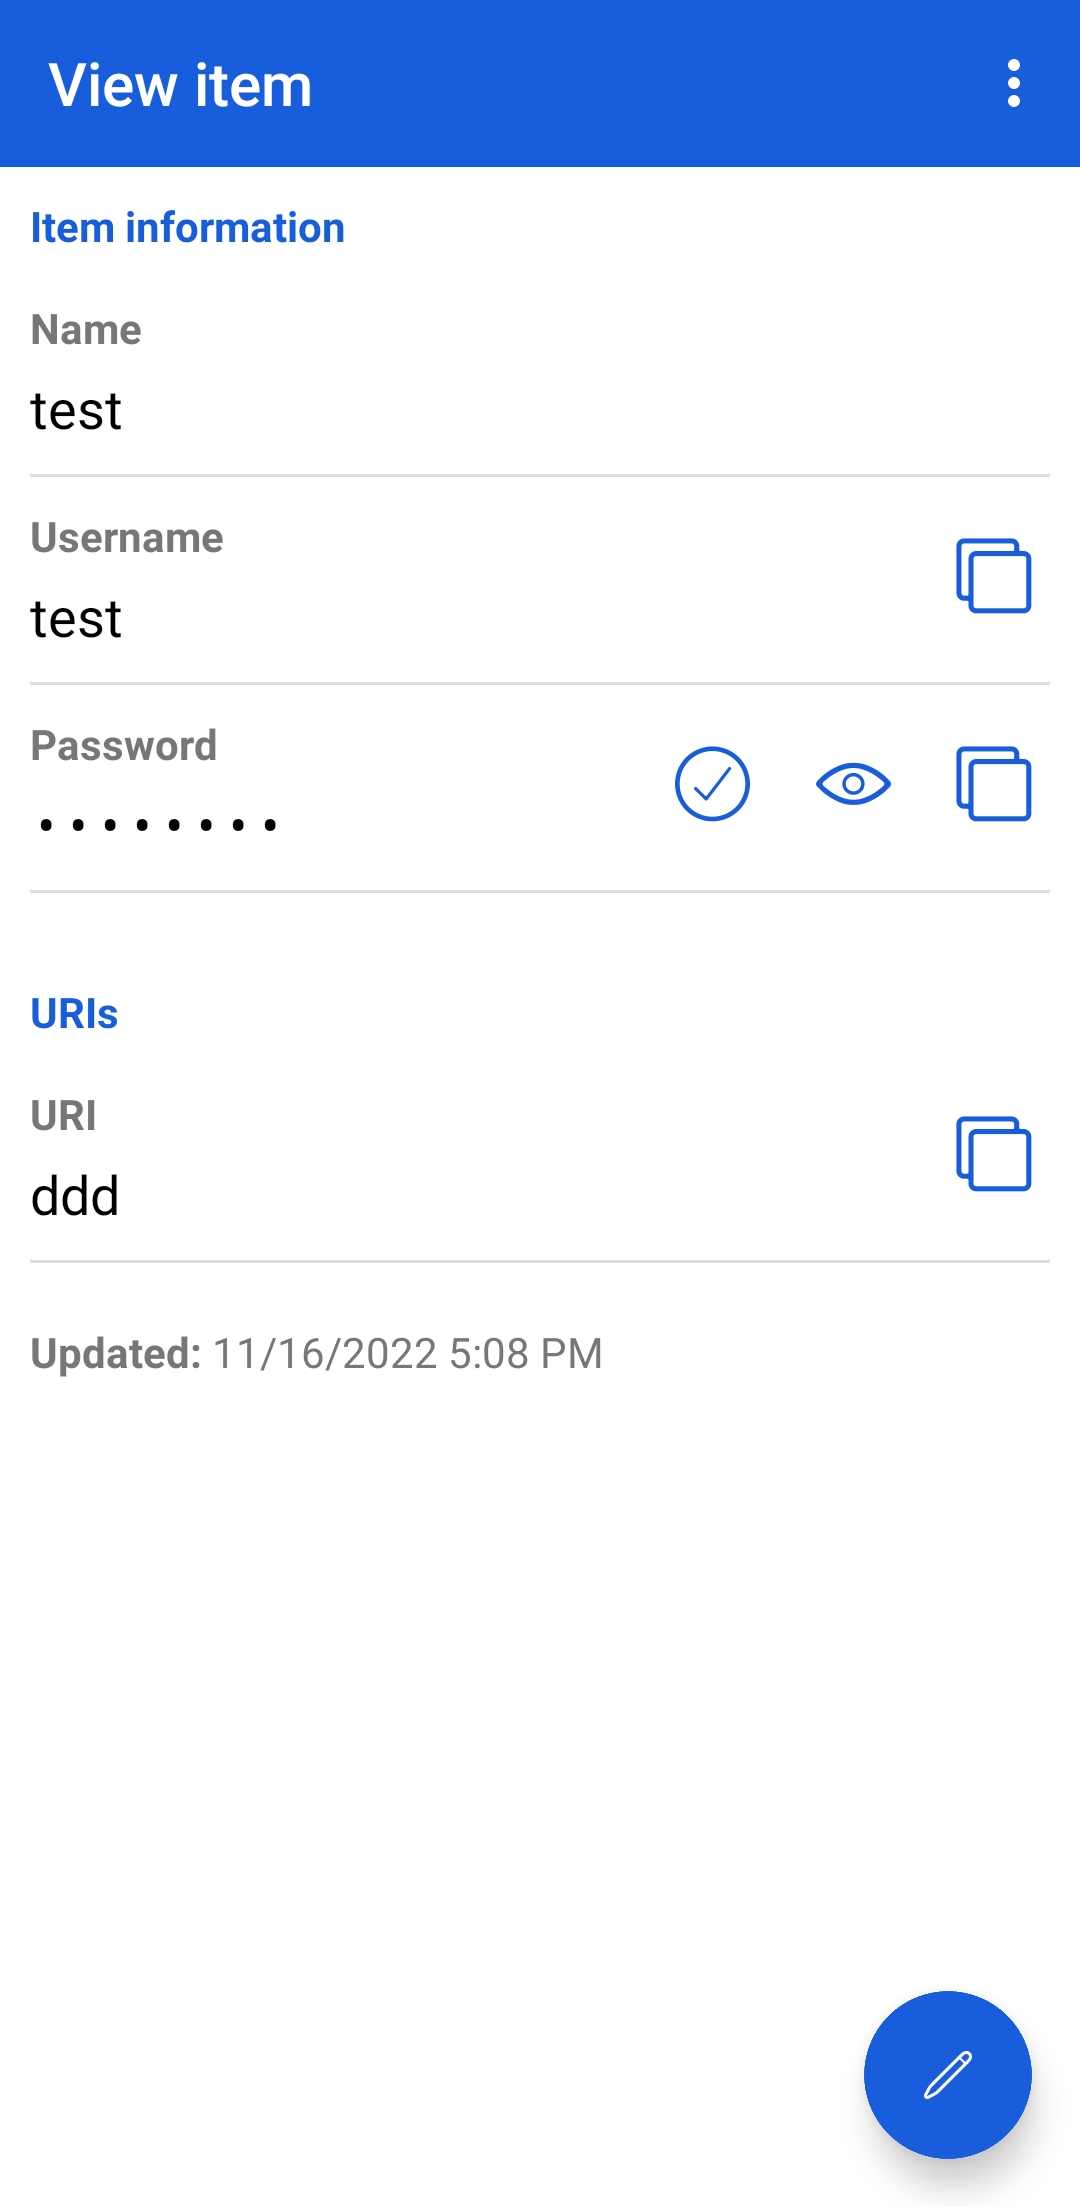
\includegraphics[width=0.4\columnwidth]{gfx/bitapp/bitapp-login-view.png}}
    \caption{pantalla de un \gls{login}. \href{https://play.google.com/store/apps/details?id=com.x8bit.bitwarden}{De la app de Bitwarden.}}
    \label{fig:bitapp-login-view}
\end{figure}

Podemos observar que el campo \textit{Password}, tiene diferentes botones, en orden de izquierda a derecha:
\begin{itemize}
    \item Comprobar clave:
    Comprueba si la clave ha sido comprometida mediante la \gls{api} de \textit{Have I Been Pwned}. \cite{pwnedpasswords}% descubierto analizando las queries con tracker control
    \item Alternar visibilidad:
    Alterna el enmascaramiento de la clave.
    \item Copiar clave:
    Copia la clave al portapapeles.
\end{itemize}
De aquí podemos extraer que cada vez que haya un botón para copiar al portapapeles es un caso de uso donde el usuario podría querer escribir de forma inalámbrica su clave. Como en la imagen no sólo hay un botón para copiar al portapapeles la clave, sino que lo hay también para el usuario y el \gls{uri} podemos entender que sería útil escribir inalámbricamente también estos campos. Por lo que ahora en el proyecto para lograr uno de los objetivos deberemos tener en cuenta dichas situaciones. Pasaremos pues a buscar en todas las pantallas de la aplicación, cuáles tienen botones para copiar al portapapeles. Esto además mejora la comodidad del producto, pues ni siquiera nos habíamos planteado la opción de enviar el \gls{uri}, lo cual si bien no ahorra mucho tiempo, el poco que ahorra hace que la interacción sea fluida, lo cual, consideramos extremadamente importante.

\begin{figure}[H]
    \centering
    \subfigure[]{\frame{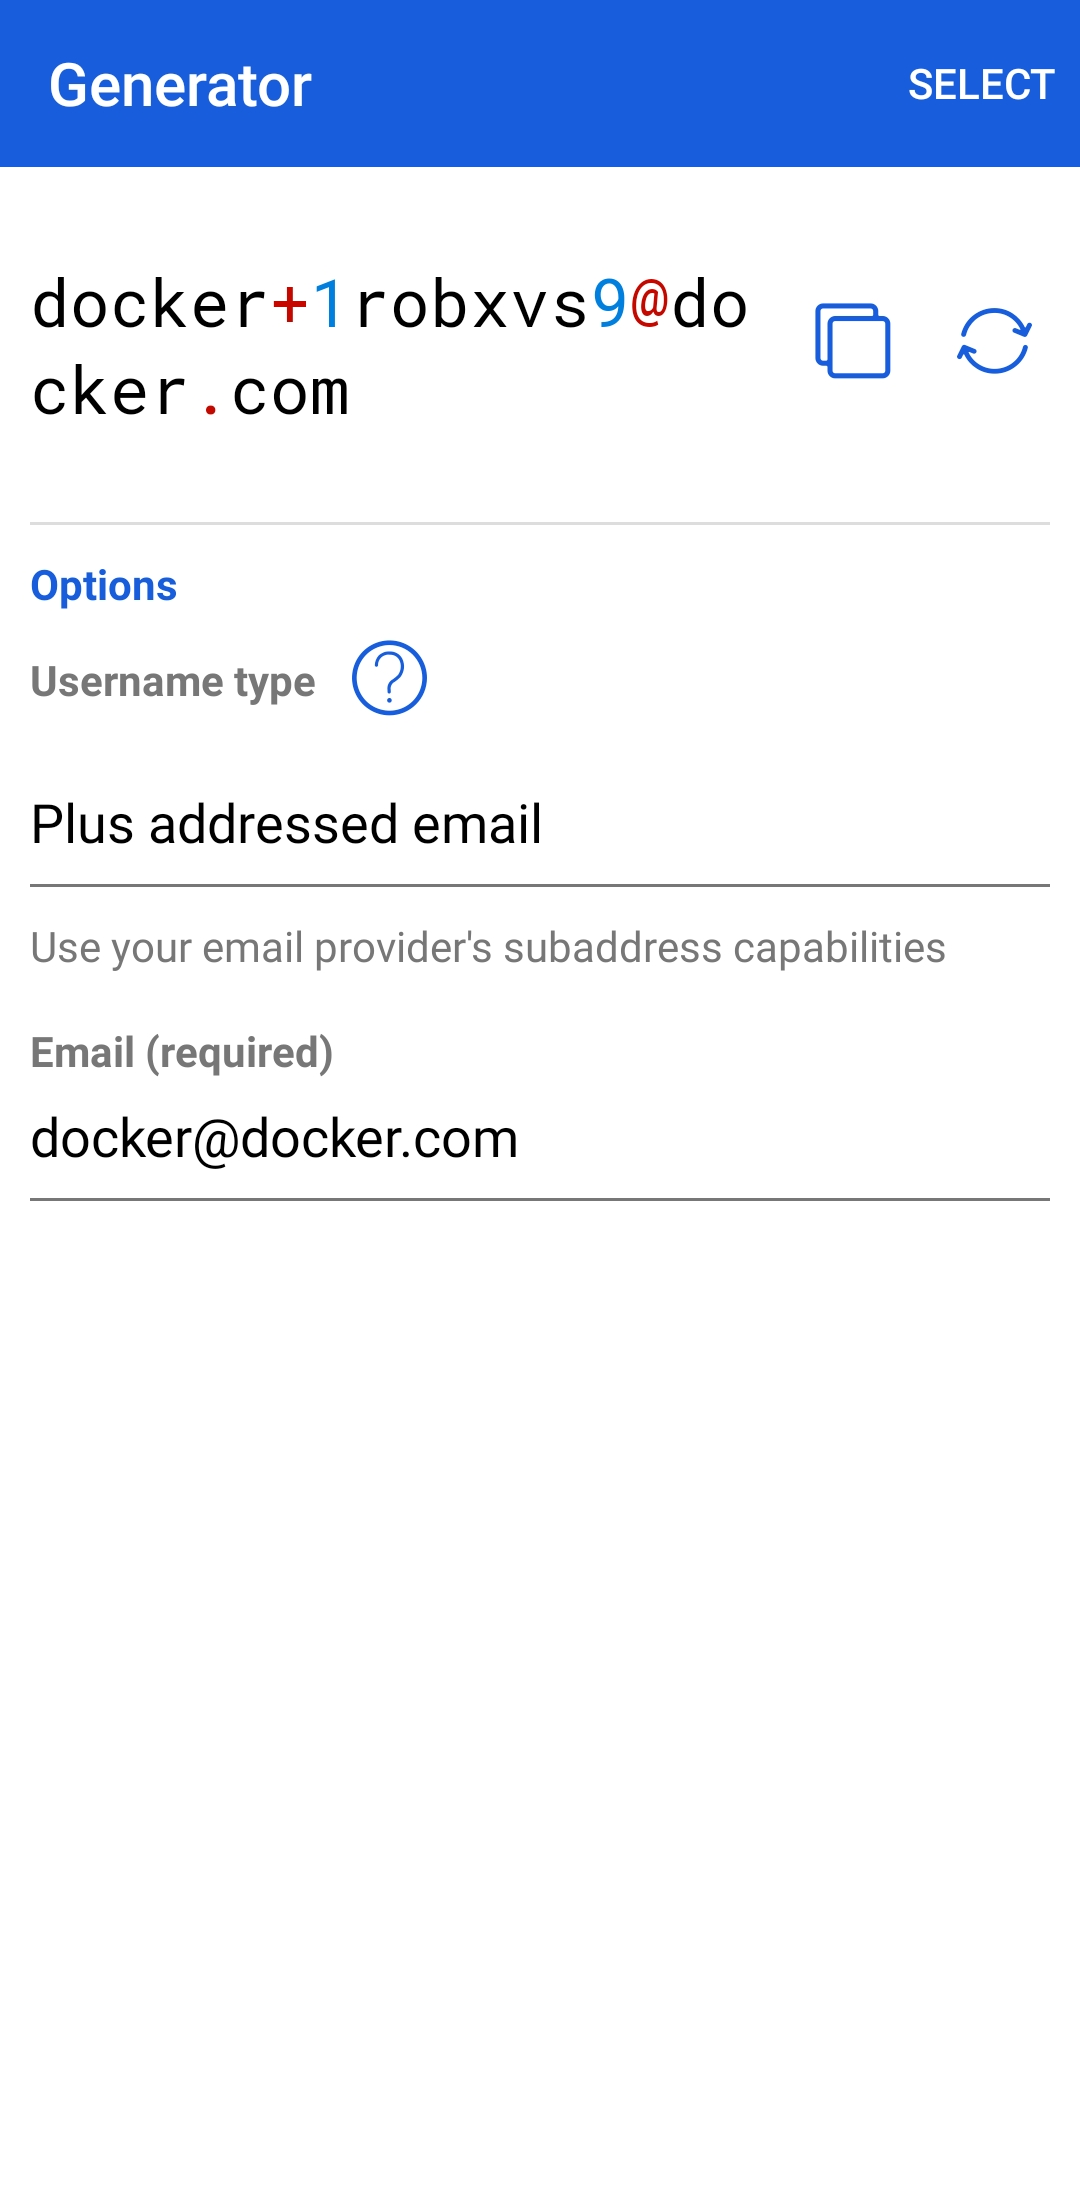
\includegraphics[width=0.24\columnwidth]{gfx/bitapp/bitapp-alias-generator-forced}}}
    \subfigure[]{\frame{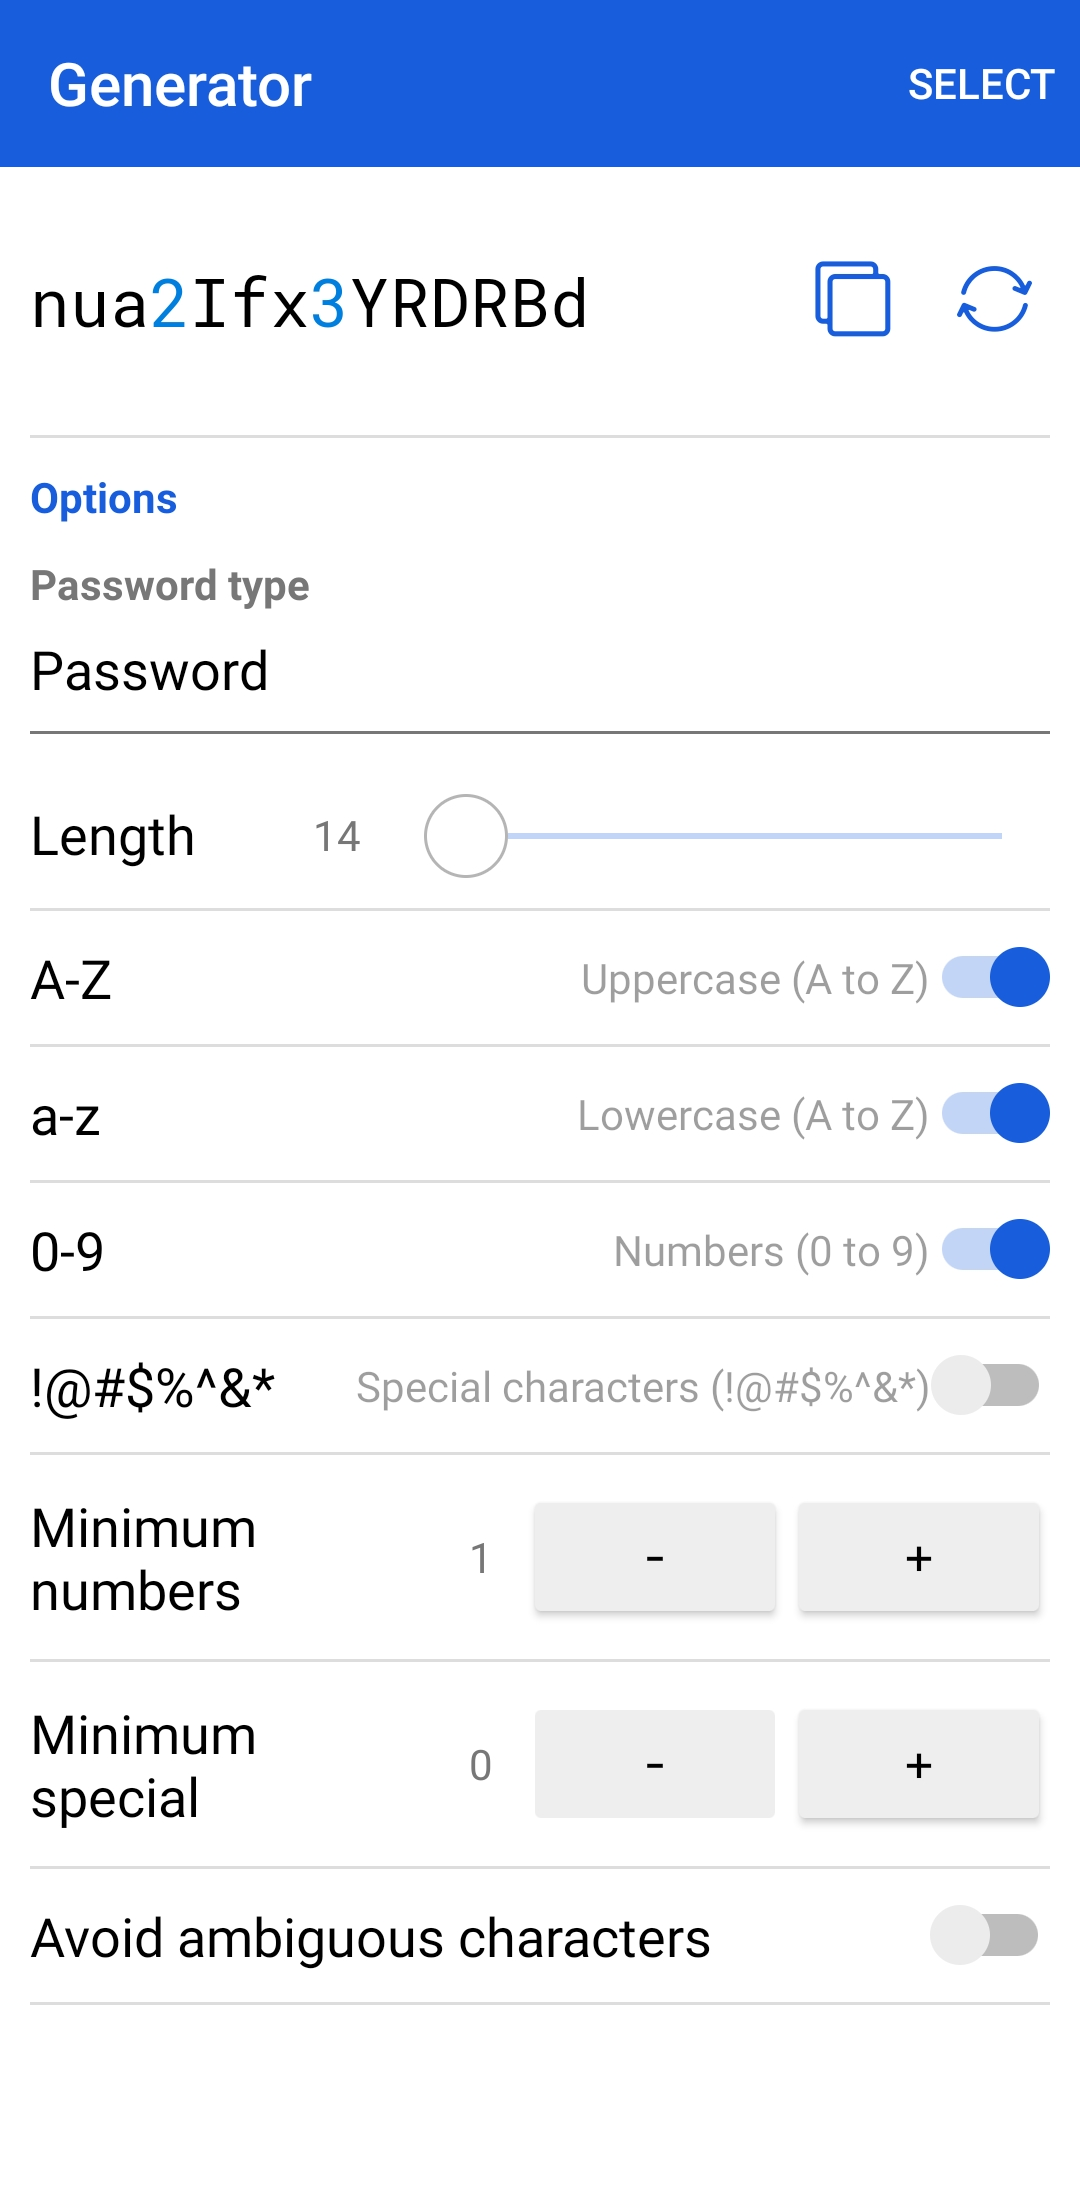
\includegraphics[width=0.24\columnwidth]{gfx/bitapp/bitapp-password-generator-forced}}}
    \subfigure[]{\frame{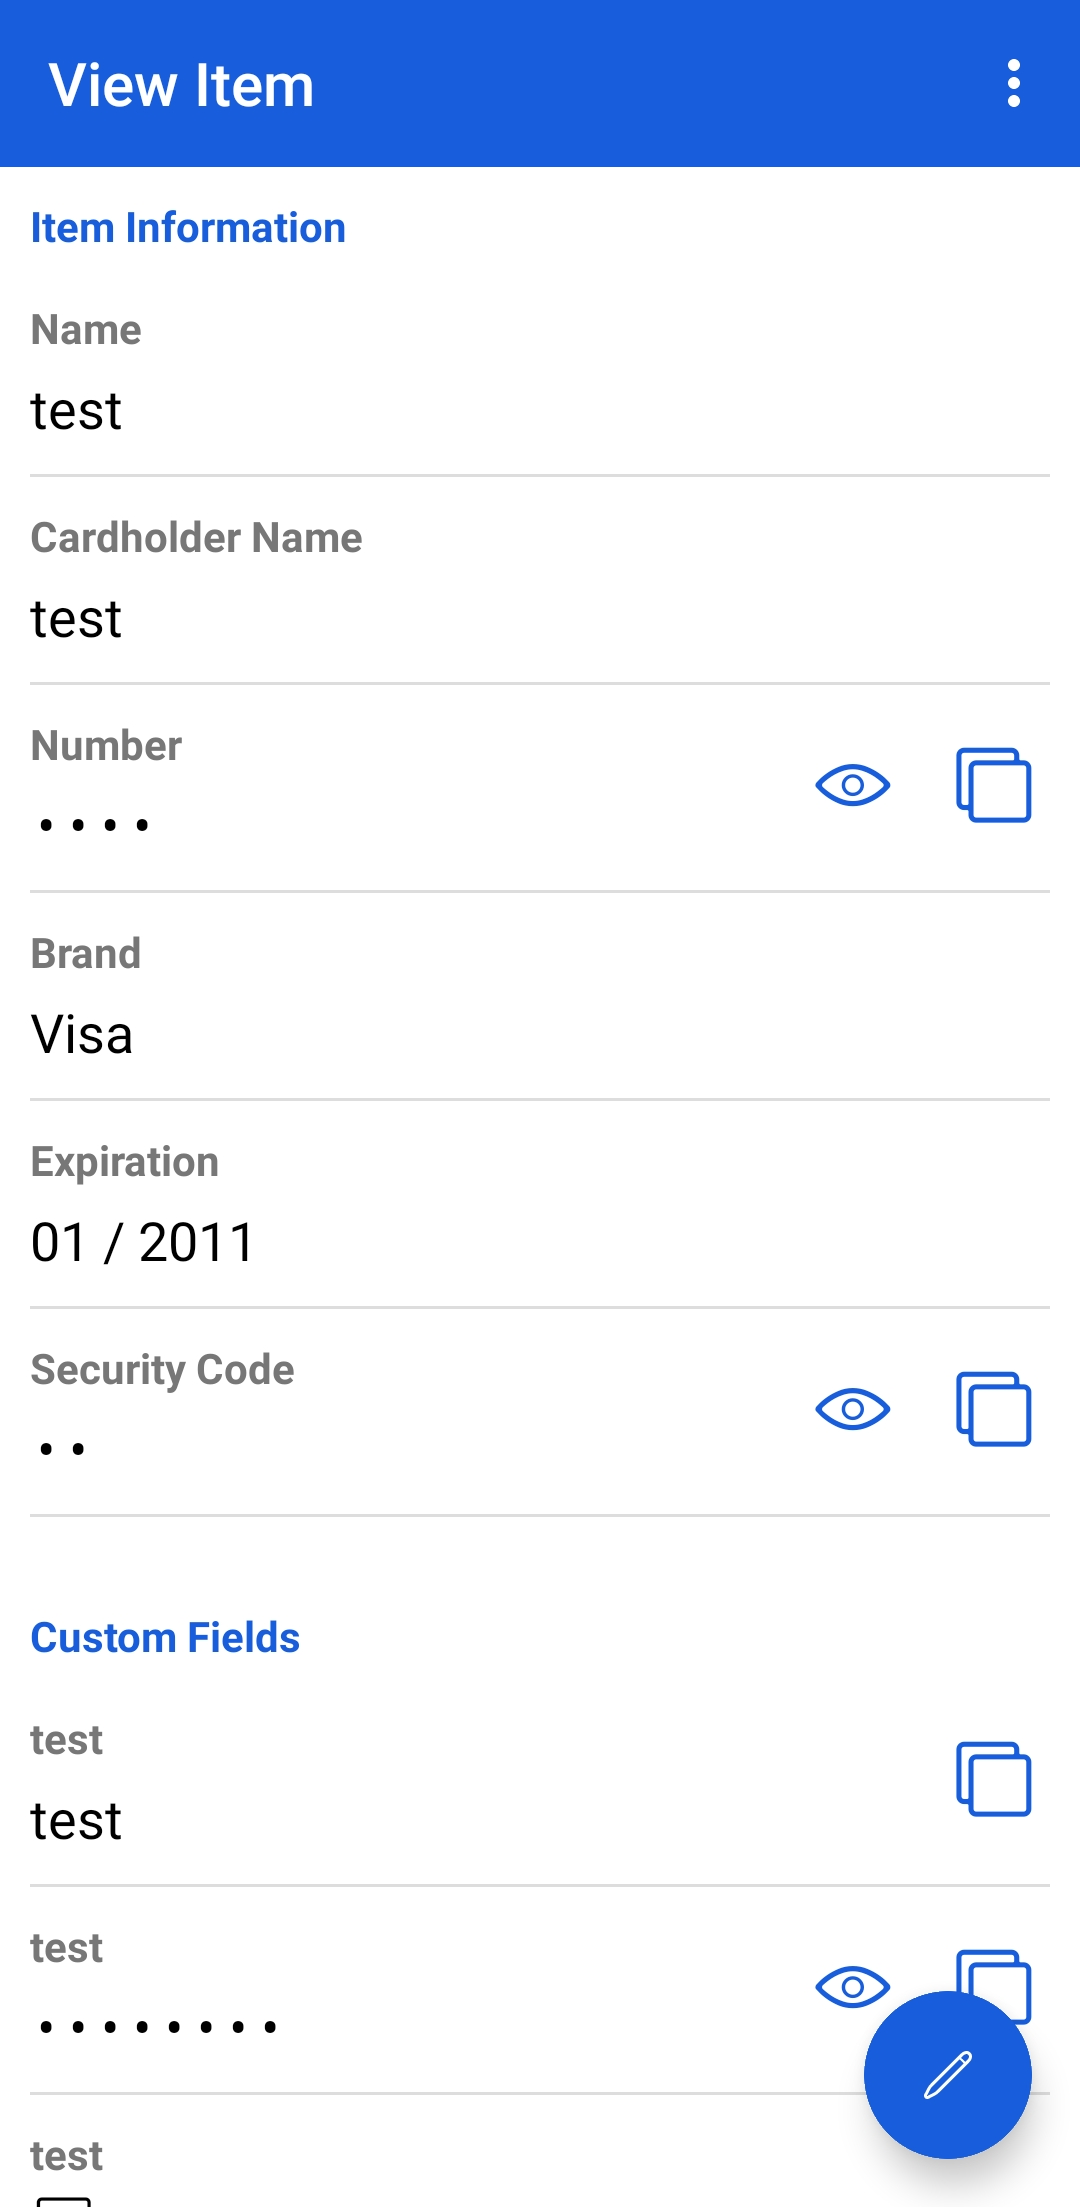
\includegraphics[width=0.24\columnwidth]{gfx/bitapp/bitapp-custom-fields-card-view}}}
    \subfigure[]{\frame{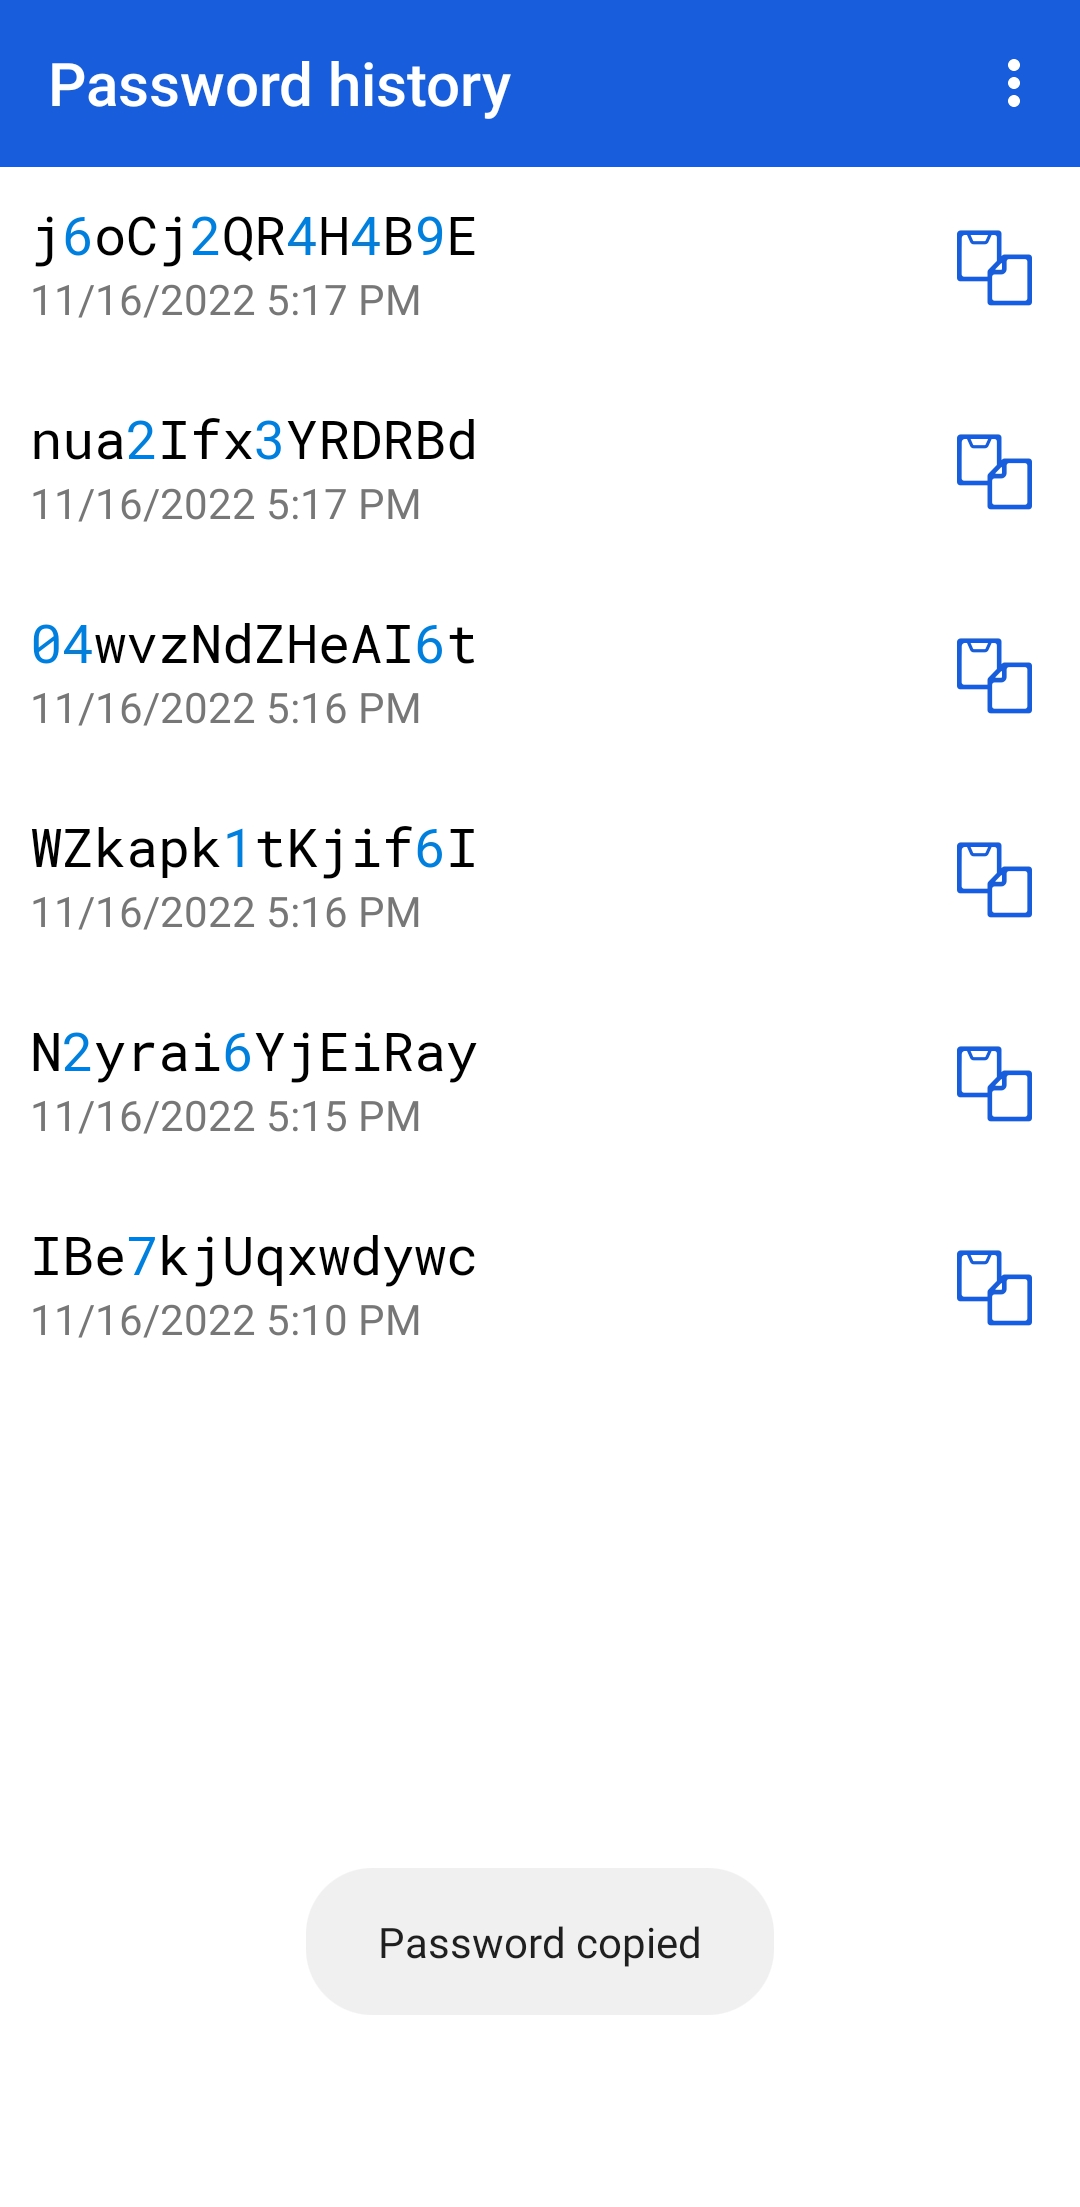
\includegraphics[width=0.24\columnwidth]{gfx/bitapp/bitapp-password-history}}}
    \caption{
        Figura múltiple. \href{https://play.google.com/store/apps/details?id=com.x8bit.bitwarden}{De la app de Bitwarden.} \newline
        \tab (a) pantalla de generación de alias. \newline
        \tab (b) pantalla de generación de claves. \newline
        \tab (c) pantalla de tarjetas, con campos adicionales. \newline
        \tab (d) pantalla de historial de claves.
        }
    \label{fig:bitapp-copy}
\end{figure}
%bitapp-custom-fields-login-view
%bitapp-generator-1-pass
%bitapp-generator-2-alias
%bitapp-password-generator-forced
%bitapp-alias-generator-forced
%bitapp-password-history

Como podemos ver en la Figura \ref{fig:bitapp-copy}, este botón lo podemos encontrar en las pantallas de generación de claves o alias, la vista de tarjeta y el historial de claves, además de la ya mencionada vista de \gls{login}. Así que estas serán las partes que modificaremos para ello.

Lo siguiente es buscar dónde añadir la configuración de InputStick, ya que es necesario poder elegir la velocidad de escritura, así como la disposición, pues el protocolo \gls{hid} no transmite caracteres, si no un código que se corresponde con la ubicación física de la tecla que se ha pulsado, el estándar usa como base una disposición de Estados Unidos, y cualquier otra disposición es en realidad o bien un mapa posición$\longleftrightarrow$carácter creado por el Sistema Operativo o bien un mapa carácter$\longleftrightarrow$posición creado por el dispositivo de entrada\cite{microsofthid}\cite{usbhid}. Como un dispositivo \gls{hid} no puede conocer este mapa, y el Sistema Operativo tampoco, el estándar es que el Sistema Operativo interpreta esta información, un teclado comunicará los códigos de las teclas, y el usuario debe ajustar en el Sistema Operativo cuál debiese ser esta, por lo general esto se hace automáticamente al configurar el idioma\cite{microsoftchangelayout}. Por ello es crucial implementar una forma de cambiar este ajuste, ya que si no se hace, habría que cambiar en el Sistema Operativo la disposición cada vez que se quiera introducir una clave con InputStick y muchas contraseñas se escribirían incorrectamente si no se cambia, pues aunque gran parte del abecedario y los números coinciden entre diferentes disposiciones, el resto de caracteres no suelen coincidir. Lo podemos ver en el siguiente ejemplo interactivo:
\begin{itemize}
    \item \hyperlink{https://learn.microsoft.com/en-us/globalization/keyboards/kbdsp}{Disposición de España.}
    \item \hyperlink{https://learn.microsoft.com/en-us/globalization/keyboards/kbdusx}{Disposición internacional de Estados Unidos.}
\end{itemize}
Si InputStick está configurado como Estados Unidos internacional, y un dispositivo Windows está configurado como España, al enviar \quotes{\#} se recibirá \quotes{·}. Aunque si el lector se anima puede probarlo usted mismo al revés, asumiendo que su teclado tiene la disposición de España. Para cambiar la configuración de la disposición en Windows 10 debe dirigirse a la pantalla de \quotes{Configuración}, en la opción \quotes{Hora e idioma},seleccione \quotes{Idioma} y ahora seleccione Inglés de Estados Unidos, si sólo puede seleccionar España tendrá que agregar un \quotes{Idioma Preferido} más abajo en la misma pantalla. Con esto al presionar \quotes{Shift} y \quotes{3}, que es equivalente a \quotes{·}, recibirá en su lugar \quotes{\#}. No olvide cambiar de nuevo su disposición a España, y eliminar el idioma que ha añadido, de lo contrario en la barra de herramientas, a la derecha, se le mostrará la disposición actual y podría cambiarlo sin querer.

En la pestaña de ajustes (Figura \ref{fig:bitapp-config}), podemos ver \textit{Auto-fill services} como un grupo independiente.
Esta funcionalidad permite auto rellenar campos de inicio de sesión en navegador y en apps del dispositivo mediante un \textit{pop-up}, tras pulsarlo se abre la \gls{vault} y el usuario puede elegir el \gls{login} que quiera.
\newpage
\begin{multicols}{2}[]
    % hardcoded, no encontré la forma de solucionarlo
    % height={0.935\textheight}
    % width={0.785\columnwidth} ya no funciona
    \begin{figure}[H]
        \centering
        \frame{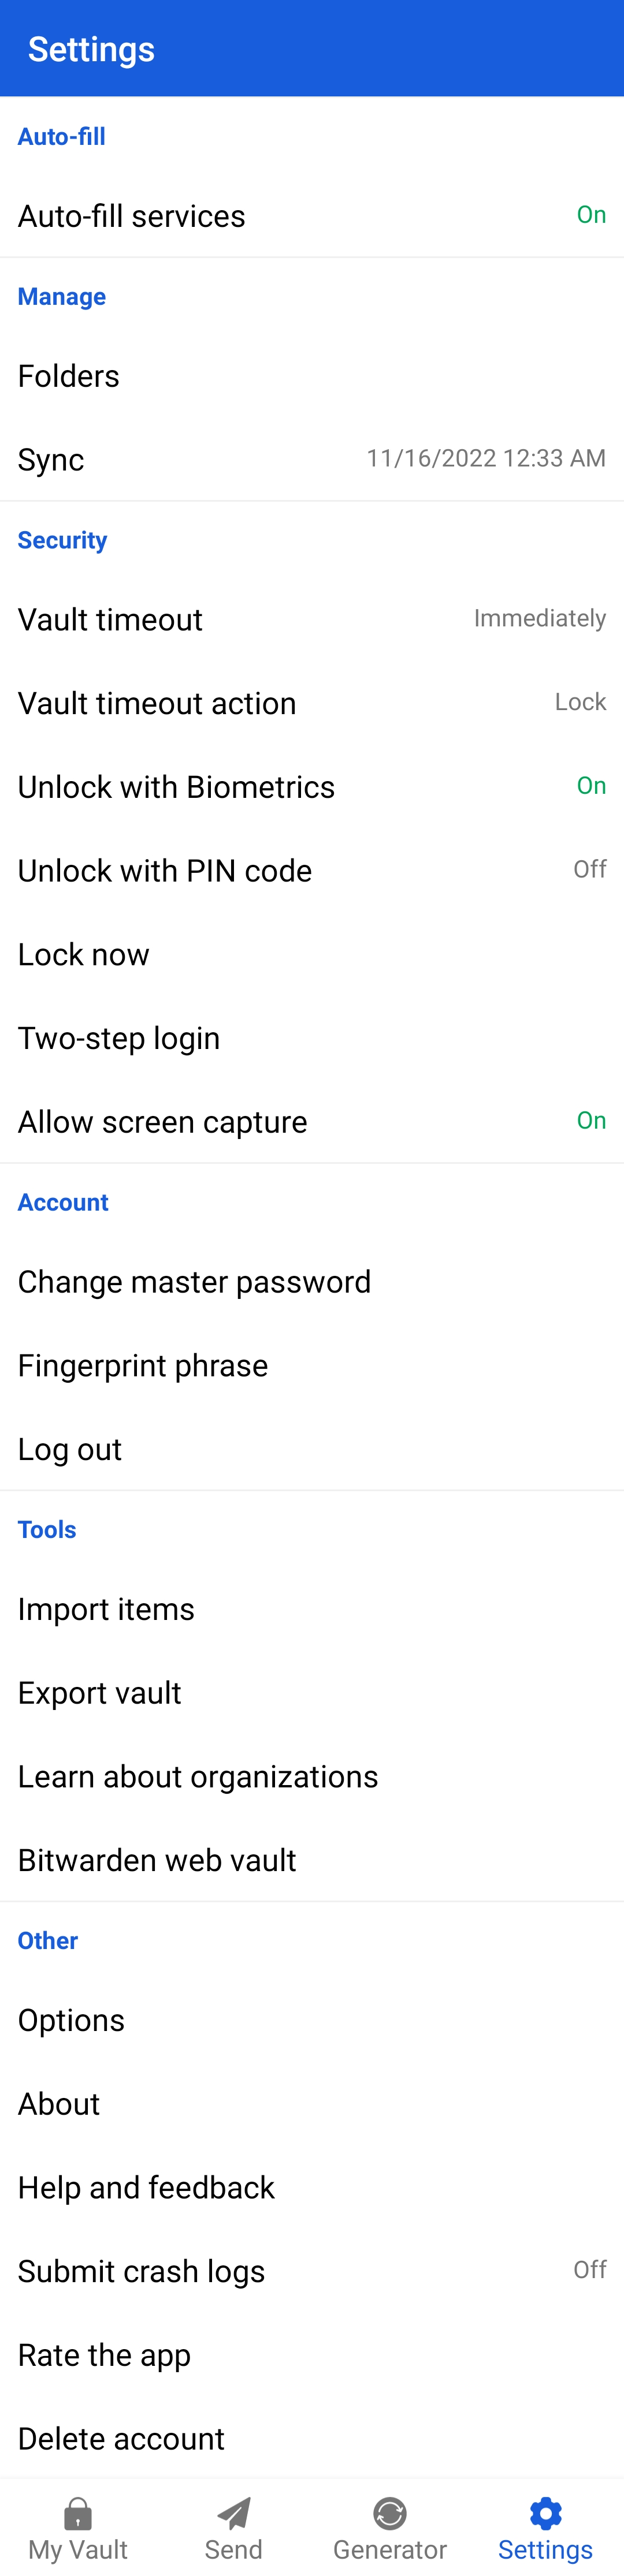
\includegraphics[height={0.935\textheight}]{gfx/bitapp/bitapp-settings-longer.png}}
        \caption{Pantalla de configuración. \href{https://play.google.com/store/apps/details?id=com.x8bit.bitwarden}{De la app de Bitwarden.}}
        \label{fig:bitapp-config}
    \end{figure}
    \columnbreak

     La funcionalidad que aporta InputStick es también un método de inicio de sesión, por lo que podríamos usar la misma estructura para este proyecto y poner la configuración en la pantalla de ajustes, debajo del servicio de auto rellenado.

    También podemos encontrar en la pantalla de Opciones (Figura \ref{fig:bitapp-options}), a la que se accede desde los ajustes, que los servicios de auto rellenado tienen también aquí parte de su configuración. Esta configuración define en qué \glspl{uri} mostrar el \textit{pop-up} del servicio de auto rellenar, también define si registrar como un \gls{login} nuevas entradas. Sin embargo la naturaleza de InputStick es distinta y no es totalmente automático, no existe esta comunicación bidireccional, siempre es unidireccional por el comportamiento del protocolo \gls{hid} mencionado anteriormente, el proceso de inicio de sesión seguirá siempre este orden:
    \begin{enumerate}
        \item Acceder al sitio donde se pretende introducir los credenciales.
        \item Poner el enfoque en el campo de texto que se quiera rellenar-
        \item En el móvil abrir la \gls{vault}.
        \item En la \gls{vault} buscar el \gls{login}.
        \item En el \gls{login} pulsar el botón de enviar.
    \end{enumerate}

    Es por ello por lo que no vamos a añadir ningún campo de configuración en esta pantalla, si no que crearemos una pantalla por separado y se accederá directamente desde la pantalla de Ajustes, teniendo así toda la configuración en la misma ubicación.

    Adicionalmente, deberemos también añadir en esa pantalla una forma de activar o desactivar el servicio, lo cual activará o desactivará los botones para enviar a InputStick.

    En resumen, los objetivos que se plantean son:
    \begin{itemize}
        \item Múltiples botones para enviar a InputStick.
        \item pantalla de ajustes con:
        \begin{itemize}
            \item Interruptor para activar o desactivar la funcionalidad.
            \item Selector de disposición.
            \item Selector de velocidad de escritura automática.
        \end{itemize}
    \end{itemize}
    \vfill\null % relleno
    \columnbreak
    \begin{figure}[H]
        \centering
        \frame{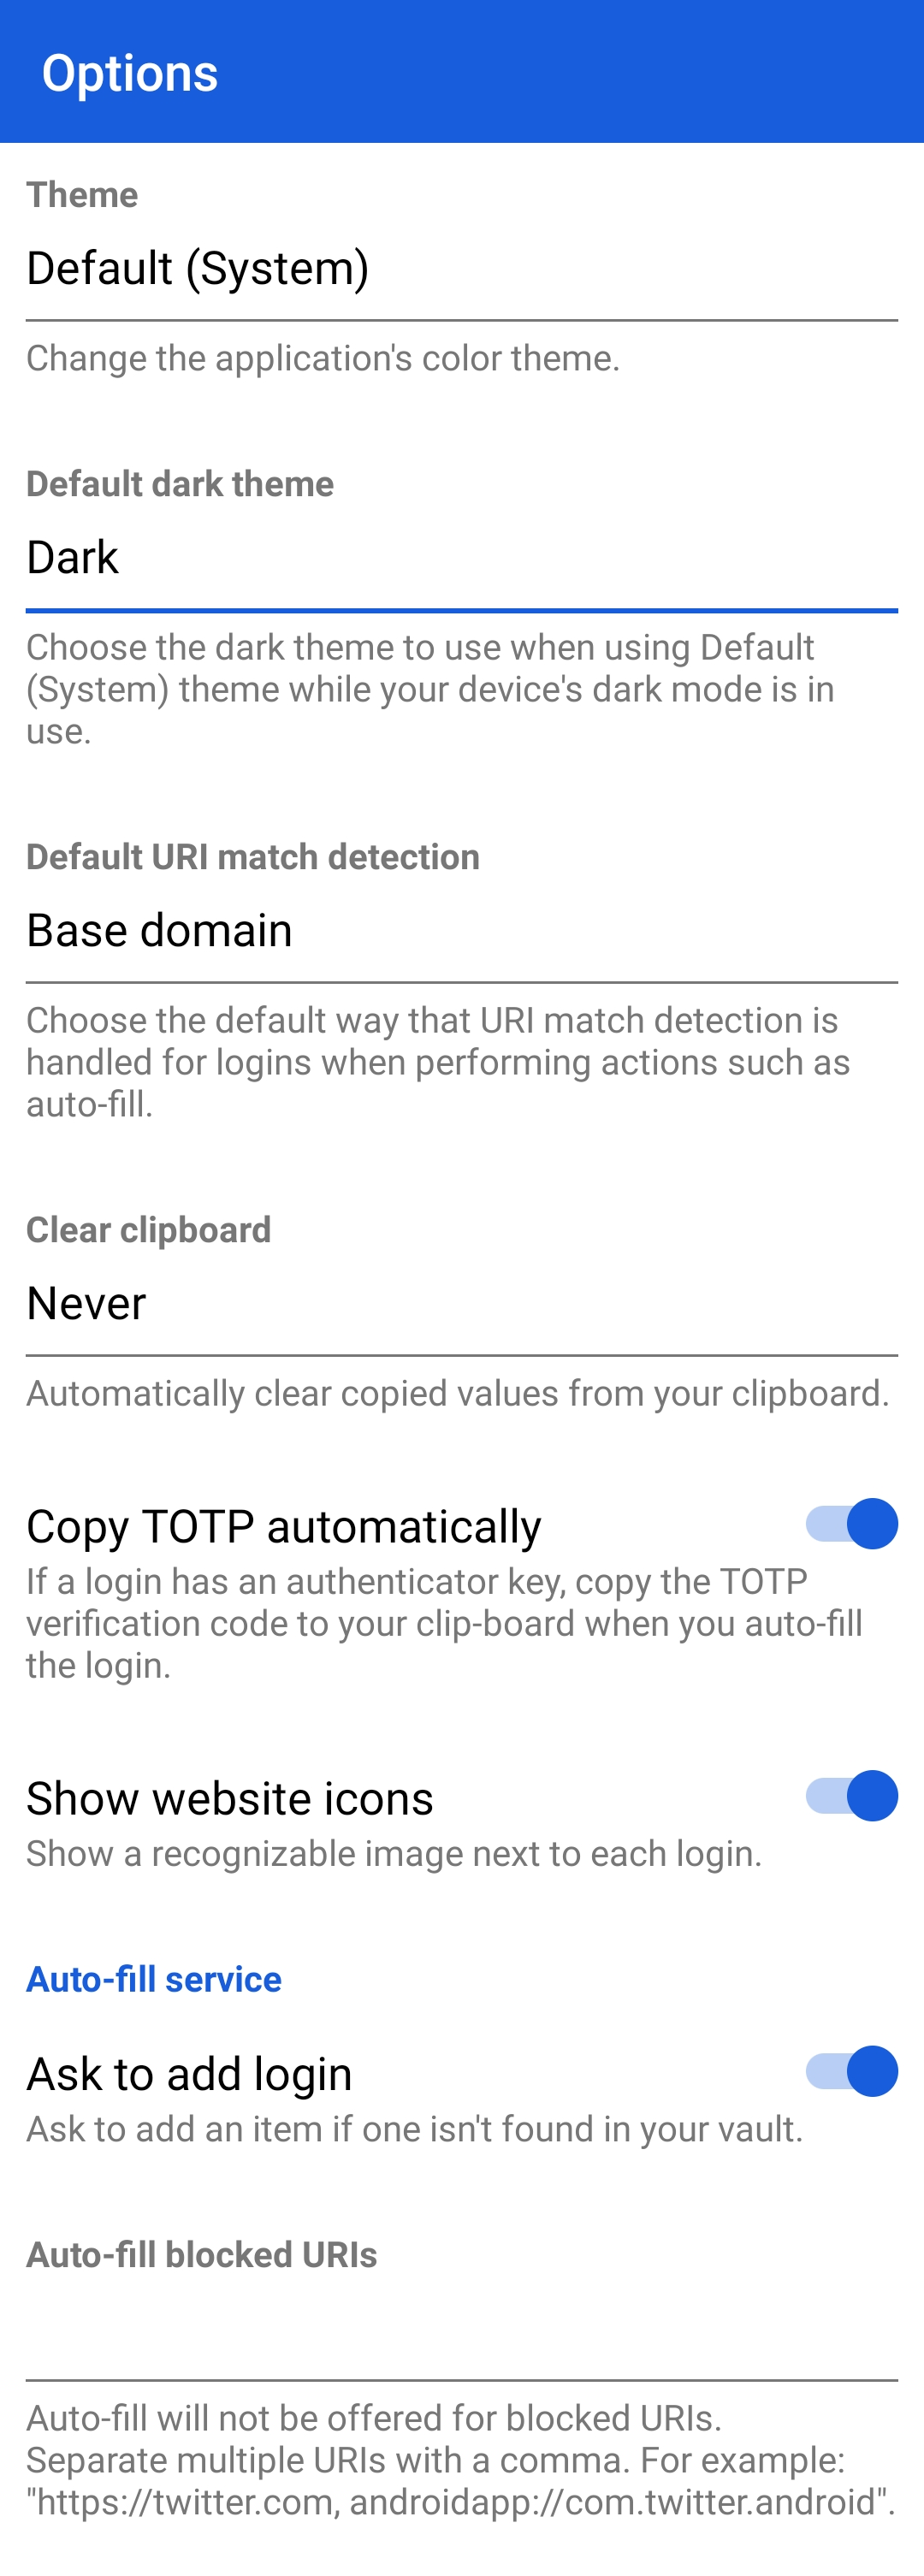
\includegraphics[width={0.785\columnwidth}]{gfx/bitapp/bitapp-options-longer.png}}
        \caption{pantalla de opciones. \href{https://play.google.com/store/apps/details?id=com.x8bit.bitwarden}{De la app de Bitwarden.}}
        \label{fig:bitapp-options}
    \end{figure}
\end{multicols}

\subsubsection{Casos de uso}
Antes de comenzar con el código, es necesario analizar los casos de uso, en la figura \ref{fig:casos} podemos ver un esquema \gls{uml} explicándolos. De forma general casos son enviar campos, elementos del generador y configurar los ajustes.
\begin{figure}[H]
    \centering
    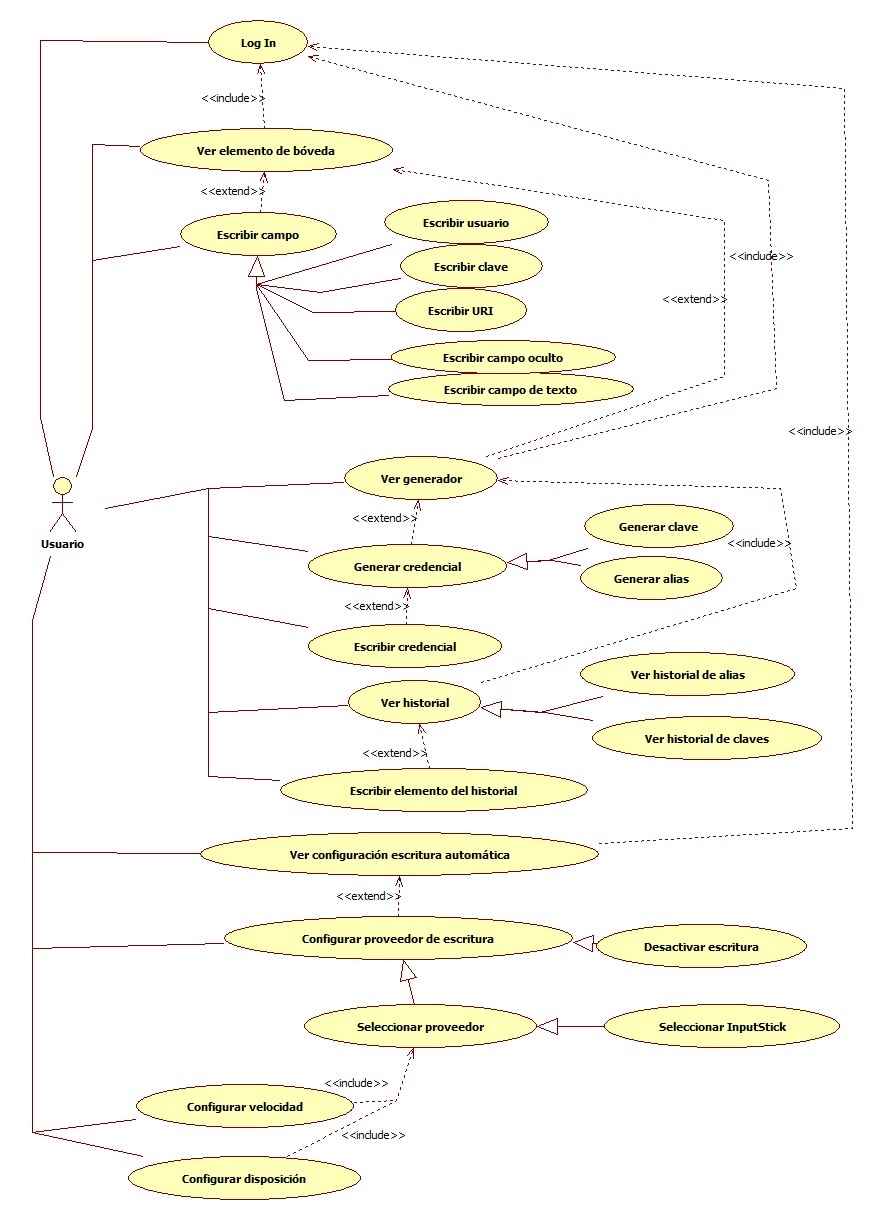
\includegraphics[height={0.935\textheight}]{gfx/casos.jpg}
    \caption{Casos de uso. Realización propia}
    \label{fig:casos}
\end{figure}


\subsubsection{Esquema}
\begin{figure}[H]
    \centering
    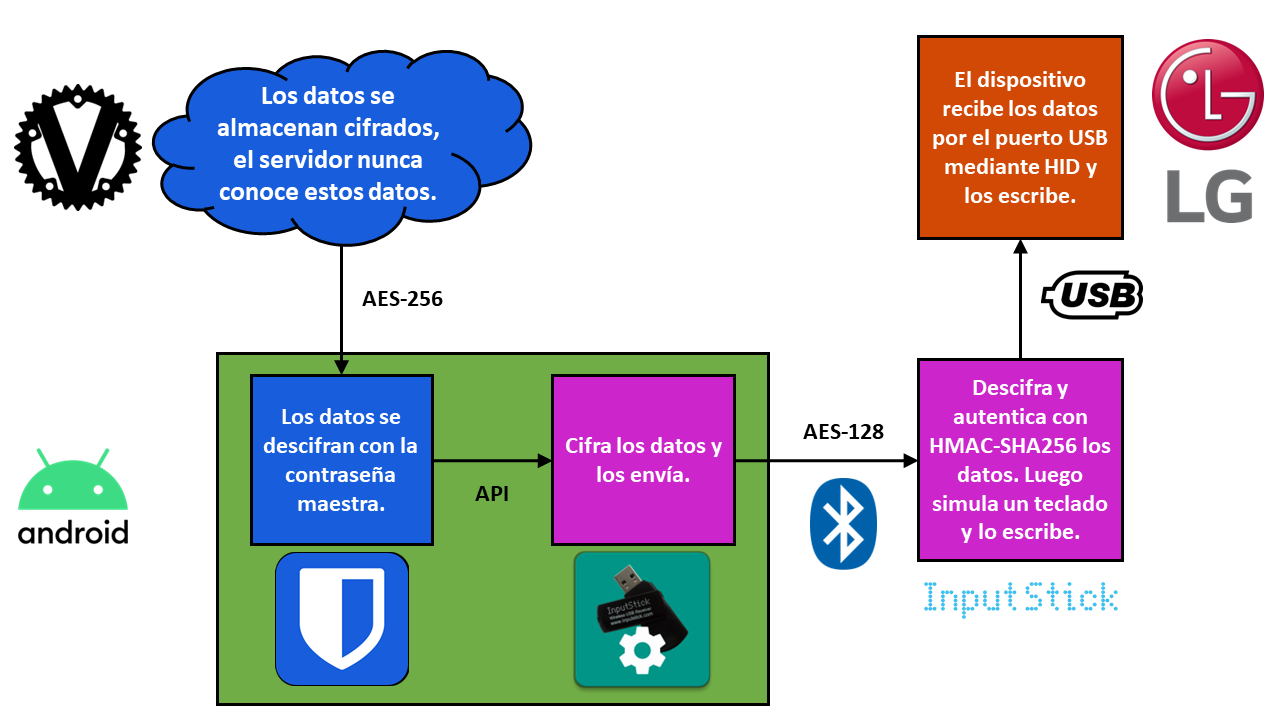
\includegraphics[width=\textwidth]{gfx/Diagrama2.png}
    \caption{Diagrama de conexiones teórico. Realización propia.}
    \label{fig:diagrama}
    El logo de LG representa una \textit{Smart TV}, a modo de ejemplo, pero es sustituible por cualquier dispositivo compatible con \gls{usb} \gls{hid}.
\end{figure}

 La figura \ref{fig:diagrama} ilustra el mapa de conexiones. El servidor de Bitwarden (en nuestro caso Vaultwarden) almacena los datos cifrados, el servidor desconoce por completo la clave para descifrarlos. Estos datos sólo son descifrados en los clientes los cuales le solicitan los datos a Bitwarden. Luego, cuando el usuario decide enviar una clave a InputStick esta se volverá a cifrar para su transmisión por Bluetooth, este proceso lo lleva la app InputStickUtility, a la cual se le transmite la información mediante la \gls{api} InputStickBroadcast\footnote{El nombre pueda dar a entender que los datos se envían a todas las apps, no es así. La llamada a \href{https://github.com/inputstick/InputStickAPI-Android/blob/81d9ce96aa9e4db4f508090f54bea981ffecfcb7/InputStickAPI/src/com/inputstick/api/broadcast/InputStickBroadcast.java\#L208}{type} llama a su vez a \href{https://github.com/inputstick/InputStickAPI-Android/blob/81d9ce96aa9e4db4f508090f54bea981ffecfcb7/InputStickAPI/src/com/inputstick/api/broadcast/InputStickBroadcast.java\#L420}{send}, aquí podemos ver que esto se envía específicamente a la app InputStickUtility.}. Cuando InputStick recibe los datos a escribir los descifra y los envía al dispositivo al que está conectado, usando el protocolo \gls{hid} por \gls{usb}. Finalmente el dispositivo lo escribe en el campo que tenga el enfoque. Se puede observar claramente como los \textbf{nunca} entran o abandonan Android \textbf{sin cifrar}, únicamente cuando se envía la información a InputStickUtility. En la figura \ref{fig:diagrama_real} se muestra como quedaría el resultado final de una forma más práctica y menos esquemática.

\begin{figure}[H]
    \centering
    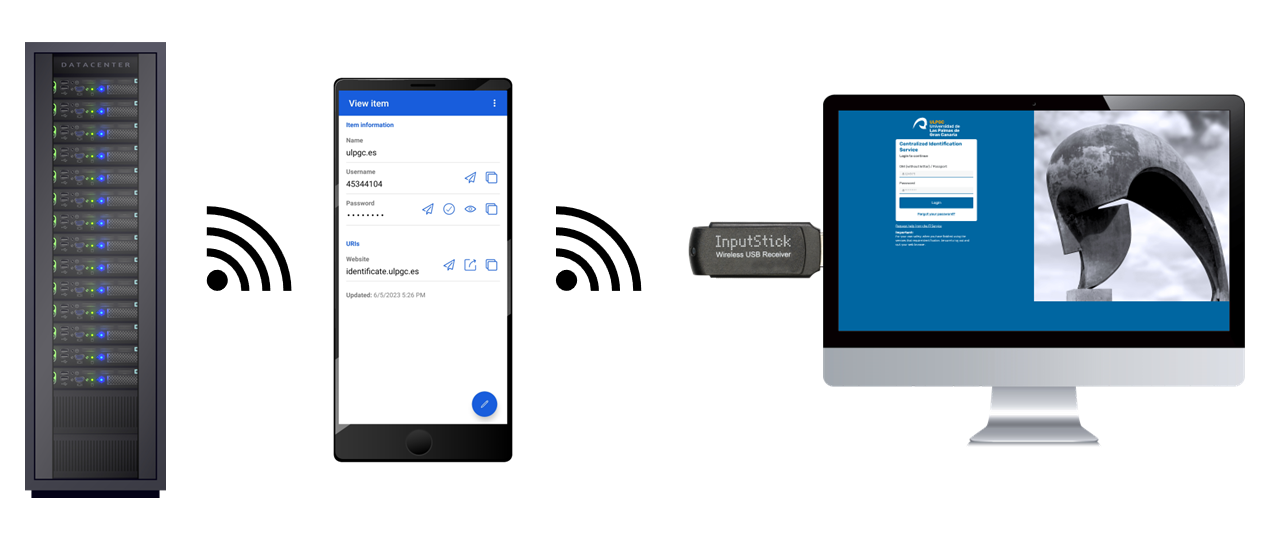
\includegraphics[width=\textwidth]{gfx/diagrama_real.png}
    \caption{Diagrama de conexiones práctico. Realización propia.}
    \label{fig:diagrama_real}
    El ordenador sobremesa es a modo de ejemplo, pero es sustituible por cualquier dispositivo compatible con \gls{usb} \gls{hid}.\newline
    Marco de móvil. Imagen por brgfx en Freepik.com.\newline
    Servidor. Imagen por macrovector en Freepik.com.\newline
    Marco de monitor. Imagen por d3images en Freepik.com.\newline
\end{figure}

% ------------------------
% ------------------------
% ------------------------
% ------------------------

\subsubsection{Model-View-ViewModel}

La app está diseñada con el patrón arquitectónico \gls{mvvm}. Como los patrones \gls{mvc} y \gls{mvp}, este patrón tiene como objetivo abstraer la vista de la lógica.
Este patrón pretende solventar problemas como el grado de acoplamiento que existe en los otros patrones, en \gls{mvc} existe poca independencia entre sus componentes, mientras que en \gls{mvp} ocurre con la vista y el presentador.
Por ello la vista modelo desconoce la existencia de la vista y el modelo desconoce la existencia de la vista modelo.
En este caso, la vista y la vista modelo están enlazadas mediante los campos de datos que son estados que indican a la vista cómo debe presentarse al usuario.
Por otro lado la vista modelo, como intermediaria, mantiene estos campos actualizados recogiendo la información necesaria del modelo, el cual se ocupa de acceder a la base de datos.\cite{García2023mvvm}\cite{Kouraklis2016}

En esta app, el uso de \gls{mvvm} hace que sea bastante fácil y cómodo desarrollarla para distintos Sistemas Operativos como es el caso de Android e iOS, y con la ayuda de Xamarin, esto resulta más claro, ya que ambas versiones comparten el código de la vista, y la vista modelo. Aunque en este proyecto nos centraremos sólo en Android.

\subsubsection{Command}

Para que la vista pueda enviar información a la vista modelo se usa el patrón de diseño command, de esta forma separan el comportamiento de un botón de la vista. Esto se logra convirtiendo solicitudes en objetos, cada objeto es una subclase de la interfaz command\cite{ulpgc.183475}\cite{García2023intro}. Todos los botones tienen una referencia en la vista al comando, el cual se encuentra declarado en la vista modelo. Curiosamente el ejemplo que se usa en libro que se cita está relacionado con el portapapeles (pegar desde el portapapeles), mientras que descubrimos que se usa el patrón command al analizar los botones anteriormente mencionados de copiar al portapapeles.

\subsubsection{Factory method}

Se usa el patrón de diseño factory method para crear diferentes versiones de campos personalizados de un \gls{login}, estos pueden ser booleanos, ocultos, de texto o relaciones. Asumimos que el objetivo es centralizar la creación de estos objetos, pues no se aprovecha el principal beneficio de este patrón, que es evitar especificar la subclase que usar, ya que se le pasa por parámetro un enumerado especificando que subclase se quiere\cite{ulpgc.183475}\cite{García2023intro}.

\subsubsection{Servicios}
La aplicación tiene un sistema de registro de servicios para fácil acceso de distintas funcionalidades en el resto de la aplicación. Se trata de un contenedor de servicios, este es una clase estática, por lo que se puede solicitar acceso a estos servicios desde cualquier parte de la aplicación. No hemos podido encontrar que patrón podría ser este, pero sospechamos que está relacionado con evitar la creación y borrado continuo de objetos.

\subsubsection{\acrfull[hyper=false]{sha}}
En concreto \gls{sha}-256, del grupo \gls{sha}-2 es una función criptográfica de hash, que se usa para verificar la integridad de un mensaje o archivo y por tanto asegurar que no ha sido alterado. Es el estándar actual debido a su eficiencia y  baja posibilidad de colisiones, que se refiere a cuando 2 mensajes distintos devuelven el mismo resultado tras aplicar la función.

\subsubsection{\acrfull[hyper=false]{hmac}}
\Gls{hmac} usa como base una función criptográfica de hash, por ejemplo \gls{sha} y lo combina con una clave simétrica. Se usa para verificar la integridad de un mensaje y por tanto asegurar que no ha sido alterado.

\subsubsection{\acrfull[hyper=false]{aes}}
Es un algoritmo simétrico de cifrado en bloque que tras diversas operaciones como sustitución y permutación cifran el mensaje o archivo. Es el estándar actual debido a su eficiencia y resistencia.
\subsection{Desarrollo}
\subsubsection{Metodología}
Este proyecto se ha llevado a cabo mediante la metodología SCRUM. Por lo que semanalmente se ha procurado tener un producto entregable, iterando en este y mejorándolo. Esto se verá reflejado en el orden de realización de tareas. Para organizar dichas tareas se ha usado Obsidian con el plugin Kanban, así se mantiene el orden de las mismas, qué hay que hacer y qué queda por hacer.

\subsubsection{Librería de InputStick}
Para la comunicación con InputStick es necesario importar la librería de InputStick\cite{sticklibrary} al proyecto. Como está escrita en Java y la aplicación de Bitwarden está escrita en Xamarin (C\#) habrá que usar un intermediaro para realizar la comunicación, para esto usaremos \gls{jbl}\cite{bindingjar} en VisualStudio, que nos permitirá importar el .jar que es la librería de InputStick.\footnote{\href{https://github.com/PabloOQ/mobile/commit/40e370ec8dcce3fb693363a26eb971239fb9728a}{Bindings library 1}, \href{https://github.com/PabloOQ/mobile/commit/d6cccb783599da01ed99baa2ad924bea75dbf7d9}{Bindings library 2}}

\subsubsection{Código}
En esta sección hablaremos del código más relevante, hemos dejado fuera algunas partes de las implementaciones de las interfaces de las que se habla, así como la parte Vista y Vista-Modelo, sólo se discutirá el Modelo, por supuesto el resto del código se encuentra en el repositorio. \ref{repos}

El código se ha escrito desde la base de que InputStick es un proveedor de escritura automática, pero pueden haber varios. Por ello, aunque actualmente sólo haya uno, en los ajustes hay un selector del proveedor, en vez de un botón para alternar activado y desactivado. Al proveedor se le debe proporcionar toda la información necesaria cada vez que se quiere escribir, este no almacena nada, excepto lo necesario para realizar conexiones, que es específico al proveedor. Podemos verlo en su interfaz:
\begin{csharp}[firstnumber=6]{src/Core/Abstractions/IAutoTyperProvider.cs}
namespace Bit.Core.Abstractions
{
    public interface IAutoTyperProvider
    {
        void Connect();
        void Disconnect();
        void Type(string text, LayoutType layout, SpeedType speed);
    }
}
\end{csharp}

Así que hemos creado un servicio AutoTyper, este servicio se ocupa de guardar y cargar datos persistentes, aunque realmente es un intermediario, así puede interceptar la información, y validarla. Esto lo hacemos por si un proveedor ya no es compatible con una disposición o se elimina el soporte para un proveedor. Si esta información es errónea o nunca ha sido configurada por el usuario se le otorga un valor por defecto.

\begin{csharp}[firstnumber=7]{src/Core/Abstractions/IAutoTyperService.cs}
namespace Bit.Core.Abstractions
{
    public interface IAutoTyperService
    {
        IAutoTyperWrapper GetTyperWrapper();

        Task InitAsync();

        Task<AutoTyperProviderType> GetProviderTypeAsync();
        Task SetProviderAsync(AutoTyperProviderType type);
        Task<LayoutType> GetLayoutAsync(AutoTyperProviderType type);
        Task SetLayoutAsync(LayoutType layout, AutoTyperProviderType type);
        Task<SpeedType> GetSpeedAsync(AutoTyperProviderType type);
        Task SetSpeedAsync(SpeedType speed, AutoTyperProviderType type);

        List<AutoTyperProviderType> GetCompatibleProviders();
        List<LayoutType> GetCompatibleLayouts(AutoTyperProviderType type);
        List<SpeedType> GetCompatibleSpeeds(AutoTyperProviderType type);

        IAutoTyperProvider CreateTyper(AutoTyperProviderType? type);
        AutoTyperProviderType ProviderType(IAutoTyperProvider? provider);
    }
}
\end{csharp}

Aquí el proveedor de auto escritura se asegura de devolver datos válidos:
\begin{csharp}[firstnumber=32]{src/Android/Services/AutoTypers/AutoTyperService.cs}
...
    public async Task<AutoTyperProviderType> GetProviderTypeAsync()
    {
        var provider = (AutoTyperProviderType?) await _stateService.GetAutoTyperProviderAsync();
        return provider ?? AutoTyperProviderType.None;
    }
...
\end{csharp}

El servicio de estados es el que realmente se ocupa de guardar los datos, los cuales son locales, pero individuales a cada cuenta en el dispositivo, este al recoger la información se asegura que esté definida, si no lo está devuelve nulo y se le relega solucionar el problema a quien realiza la llamada, que siempre es nuestro servicio intermediaro AutoTyper.
\begin{csharp}[firstnumber=1318]{src/Core/Services/StateService.cs}
...
    public async Task<int?> GetAutoTyperProviderAsync(string userId = null)
    {
        var reconciledOptions = ReconcileOptions(new StorageOptions { UserId = userId },
            await GetDefaultStorageOptionsAsync());
        var key = Constants.AutoTyperProviderKey(reconciledOptions.UserId);
        int? provider = await GetValueAsync<int?>(key, reconciledOptions);
        // Check if provider is valid
        if (provider != null && !Enum.IsDefined(typeof(AutoTyperProviderType), (byte)provider))
        {
            provider = null;
        }
        return provider;
    }
...
\end{csharp}

Adicionalmente al recoger las disposiciones y velocidades siempre se debe devolver un valor concreto, no existe \quotes{Ninguna disposición} ni \quotes{Ninguna velocidad}. Por ello el servicio de auto escritura se solicita a sí mismo las opciones compatibles y contrasta el valor por defecto con esta lista, ya que un proveedor puede no ser compatible con ese valor, si no lo es elegimos un valor cualquiera, en este caso el primer elemento de la lista.

\begin{csharp}[firstnumber=107]{src/Android/Services/AutoTypers/AutoTyperService.cs}
...
        // Helpers

        /**
         * Checks if the element is in the list
         * If not, it defaults to def
         * If def is not in the list, it defaults to the first element of the list  
         */
        private static T Validate<T>(T element, List<T> list, T def)
        {
            return FindOrDefault(FindOrDefault(element, list, def), list, list[0]);
        }

        /**
         * Checks if the element is in the list
         * If not, it defaults to def
         */
        private static T FindOrDefault<T>(T element, List<T> list, T def)
        {
            return list.Contains(element) ? element : def;
        }
    }
}
\end{csharp}


Al servicio de auto escritura se le puede solicitar un contenedor de proveedor, esta es la única forma de contactar con el proveedor, así forzamos a que cuando se vaya a enviar algo para escribir al proveedor los datos ya hayan sido inicializados (proveedor, distribución y velocidad). Y aunque pueden haber varias instancias de la implementación del contenedor, el servicio devolverá siempre la misma instancia cuando se le solicite, de forma similar al patrón singleton, ya que el contenedor actua como una extensión del servicio.
\begin{csharp}[firstnumber=3]{src/Core/Abstractions/IAutoTyperWrapper.cs}
namespace Bit.Core.Abstractions
{
    public interface IAutoTyperWrapper
    {
        Task LoadAsync();
        void Connect();
        void Disconnect();
        void Type(string text);
        bool IsEnabled();
    }
}
\end{csharp}

En nuestro caso hemos usado la librería de InputStick mediante llamadas a la app de InputStickUtility, que se ocupa de mandar los datos a InputStick. Lamentablemente no es lo que se pretendía, pero la falta de tiempo nos ha impedido usar la \gls{api} de InputStick en mayor profundidad. Dicha \gls{api} se puede usar de dos formas:
\begin{itemize}
    \item InputStickBroadcast: Al usar esta parte de la \gls{api} es mucho más simple contactar con InputStick, ya que únicamente es necesario mandar a InputStick qué tiene que escribir, del resto se ocupa InputStickUtility.
    \item Completa: Al usar la \gls{api} en su totalidad se puede evitar la instalación de InputStickUtility, pero es requiere una implementación más compleja ya que las facilidades que otorgaba InputStickUtility ya no están presentes, por ejemplo es necesario saber la dirección \textit{Media Access Control}(MAC)\footnote{Esta es la única vez en este documento que usaremos el acrónimo MAC con un significado distinto a \acrlong{cryptomac}} de InputStick.
\end{itemize}
\begin{csharp}[firstnumber=9]{src/Android/Services/AutoTypers/InputStickBroadcastAndroid.cs}
namespace Bit.Droid.Services.AutoTypers
{
    public class InputStickBroadcastAndroid : IAutoTyperProvider
    {
        public void Connect()
        {
            InputStickBroadcast.RequestConnection(Application.Context);
        }

        public void Disconnect()
        {
            InputStickBroadcast.ReleaseConnection(Application.Context);
        }

        public void Type(String text, LayoutType layout, SpeedType speed)
        {
            InputStickBroadcast.Type(Application.Context,
                text,
                _layouts.ContainsKey(layout) ? _layouts[layout] : _layouts[0], // Should not happen, this is a fallback
                SpeedToValue(speed));
        }
...
\end{csharp}


Para administrar la selección de distribución se usa un enum, este enum contiene todas las disposiciones listadas por InputStick:
\noindent\url{https://github.com/inputstick/InputStickAPI-Android#keyboard-layouts}
\begin{csharp}[firstnumber=3]{src/Core/Enums/LayoutType.cs}
namespace Bit.Core.Enums
{
    public enum LayoutType
    {
        [LocalizableEnum("AutoTyperLayoutCSCZ")]
        cs_CZ = 0,
        [LocalizableEnum("AutoTyperLayoutDADK")]
        da_DK = 1,
...
\end{csharp}

Igualmente para administrar la velocidad de escritura se usa otro enum, este enum es una ampliación de las posibilidades que ofrece InputStick, ya que las apps oficiales de InputStick usan todas las velocidades listadas excepto \quotes{Fast} y \quotes{Faster}. De cara al usuario se usan estos términos y no las velocidades reales dos motivos:
\begin{itemize}
    \item Para no abrumar al usuario: Es innecesario que el usuario sepa las velocidades concretas, mostrar tantos números, en una escala que realmente a las velocidades más altas una persona no es capaz de cuantizar la diferencia, solo lograría sobreestimularlo.
    \item Porque realmente no es consistente: Estas velocidades se han extraído de las apps oficiales de InputStick creando un pequeño script de python en el que medir las velocidades, pues el creador no dice en ningún lugar las velocidades ya que dependen de la carga de trabajo del dispositivo en el que esté conectado. Si el dispositivo está muy sobrecargado la máxima velocidad no funcionará correctamente y el dispositivo no leerá todas las teclas y por tanto se saltará alguna. Por tanto las velocidades descritas son aproximaciones bajo poca carga.
\end{itemize}
\begin{csharp}[firstnumber=3]{src/Core/Enums/SpeedType.cs}
namespace Bit.Core.Enums
{
    public enum SpeedType : int         // keys per second (aproximate) - ratio
    {
        [LocalizableEnum("Slowest")]    // 8 - 0.1
        Slowest = 0,
        [LocalizableEnum("Slower")]     // 16 - 0.2
        Slower = 2,
        [LocalizableEnum("Slow")]       // 40 - 0.5
        Slow = 3,
        [LocalizableEnum("Normal")]     // 80 - 1
        Normal = 5,
        [LocalizableEnum("Fast")]       // 120 - 1.5
        Fast = 7,
        [LocalizableEnum("Faster")]     // 180 - 2.25
        Faster = 6,
        [LocalizableEnum("Fastest")]    // 240 - 3
        Fastest = 10,                   
    }
}
\end{csharp}
\newpage
\subsubsection{Cambios visuales}
En la figura \ref{fig:bitapp-mod} podemos ver los cambios hechos en la GUI. En cada campo que hubiese un botón de copiar al portapapeles se ha añadido el botón de enviar al proveedor de escritura automática, este campo sólo es visible cuando se ha seleccionado un proveedor. También se ha añadido una pantalla de configuración de esta funcionalidad, con selectores de proveedor, idioma y velocidad. Se puede acceder a la pantalla de los ajustes del proveedor de escritura automática desde la pantalla de ajustes.
\begin{figure}[H]
    \centering
    \subfigure[]{\frame{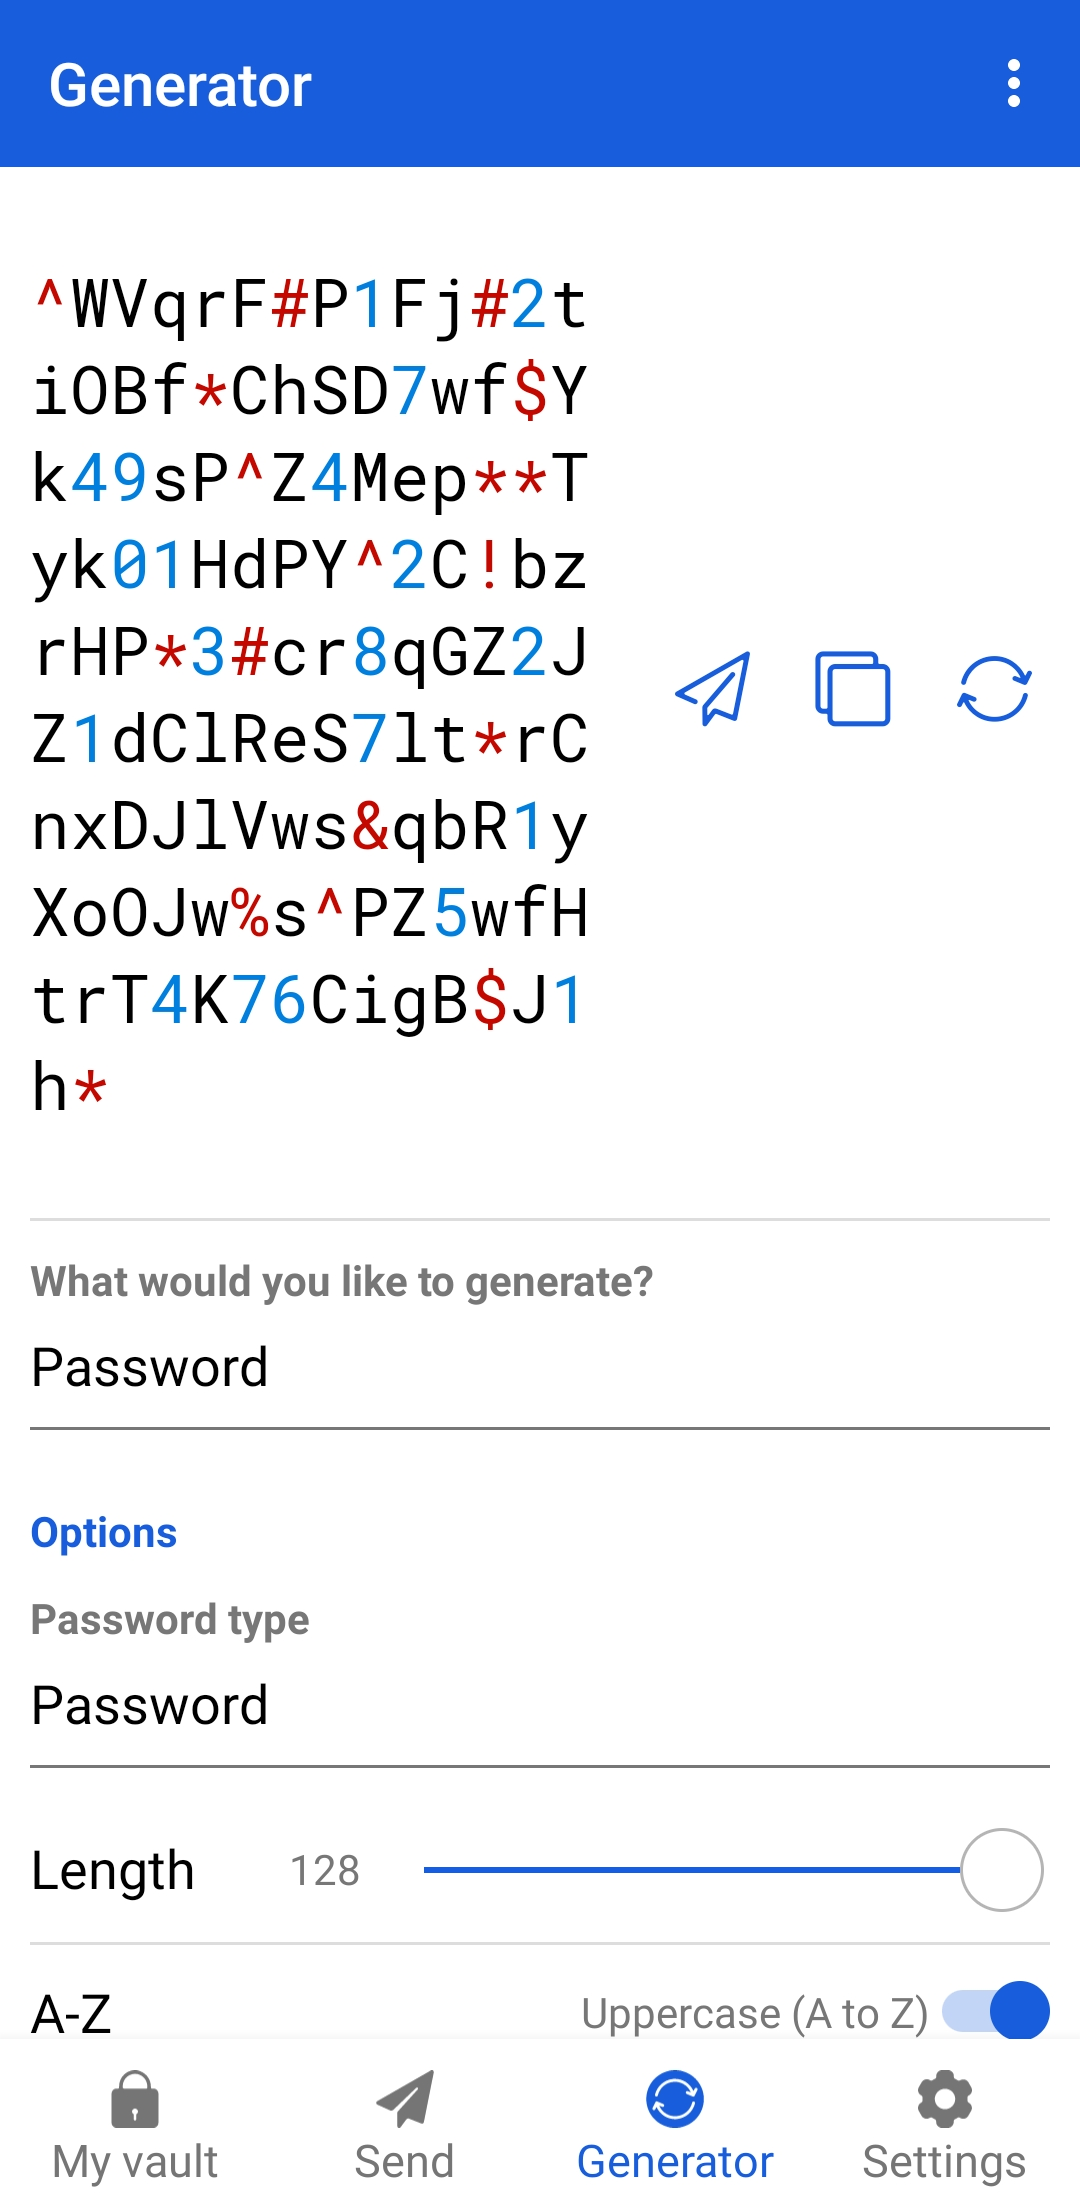
\includegraphics[width=0.4\columnwidth]{gfx/bitapp-mod-generator.png}}}
    \subfigure[]{\frame{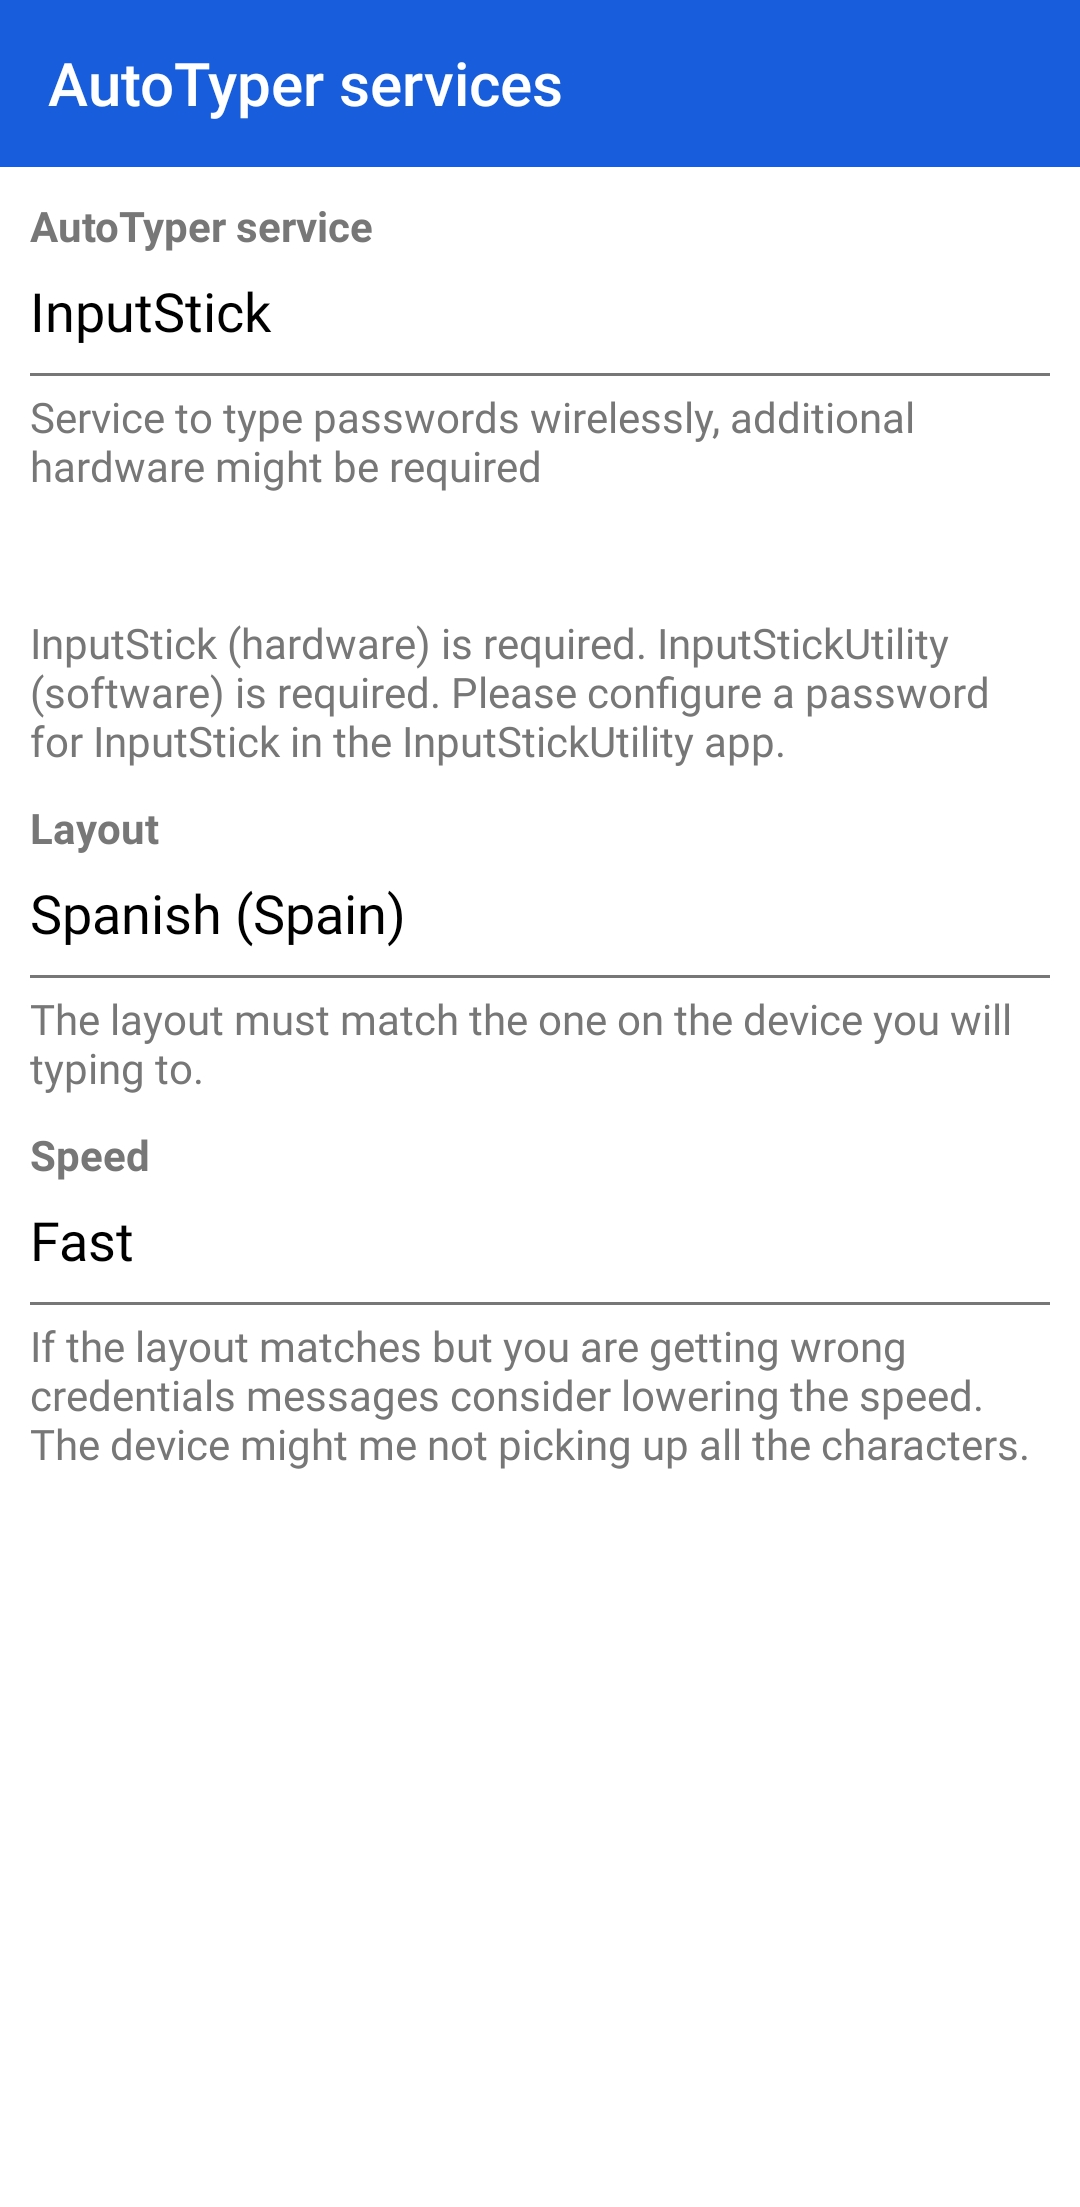
\includegraphics[width=0.4\columnwidth]{gfx/bitapp-mod-settings.png}}}
\caption{
        Figura múltiple. Modificación de la app de Bitwarden. \newline
        \tab (a) Pantalla de generación con el botón de enviar. \newline
        \tab (b) Pantalla de ajustes del proveedor de escritura automática.
        }
    \label{fig:bitapp-mod}
\end{figure}

En la figura \ref{fig:bitapp-mod-login} podemos ver todos los cambios realizados en la pantalla de un \gls{login}. El botón de enviar se encuentra en varios campos, hay que destacar que si un campo se encuentra vacío no hay nada que enviar, por lo que no se mostraría. Tampoco se mostraría si el proveedor de escritura automática se encuentra desactivado.
\begin{figure}[H]
    \centering
    \frame{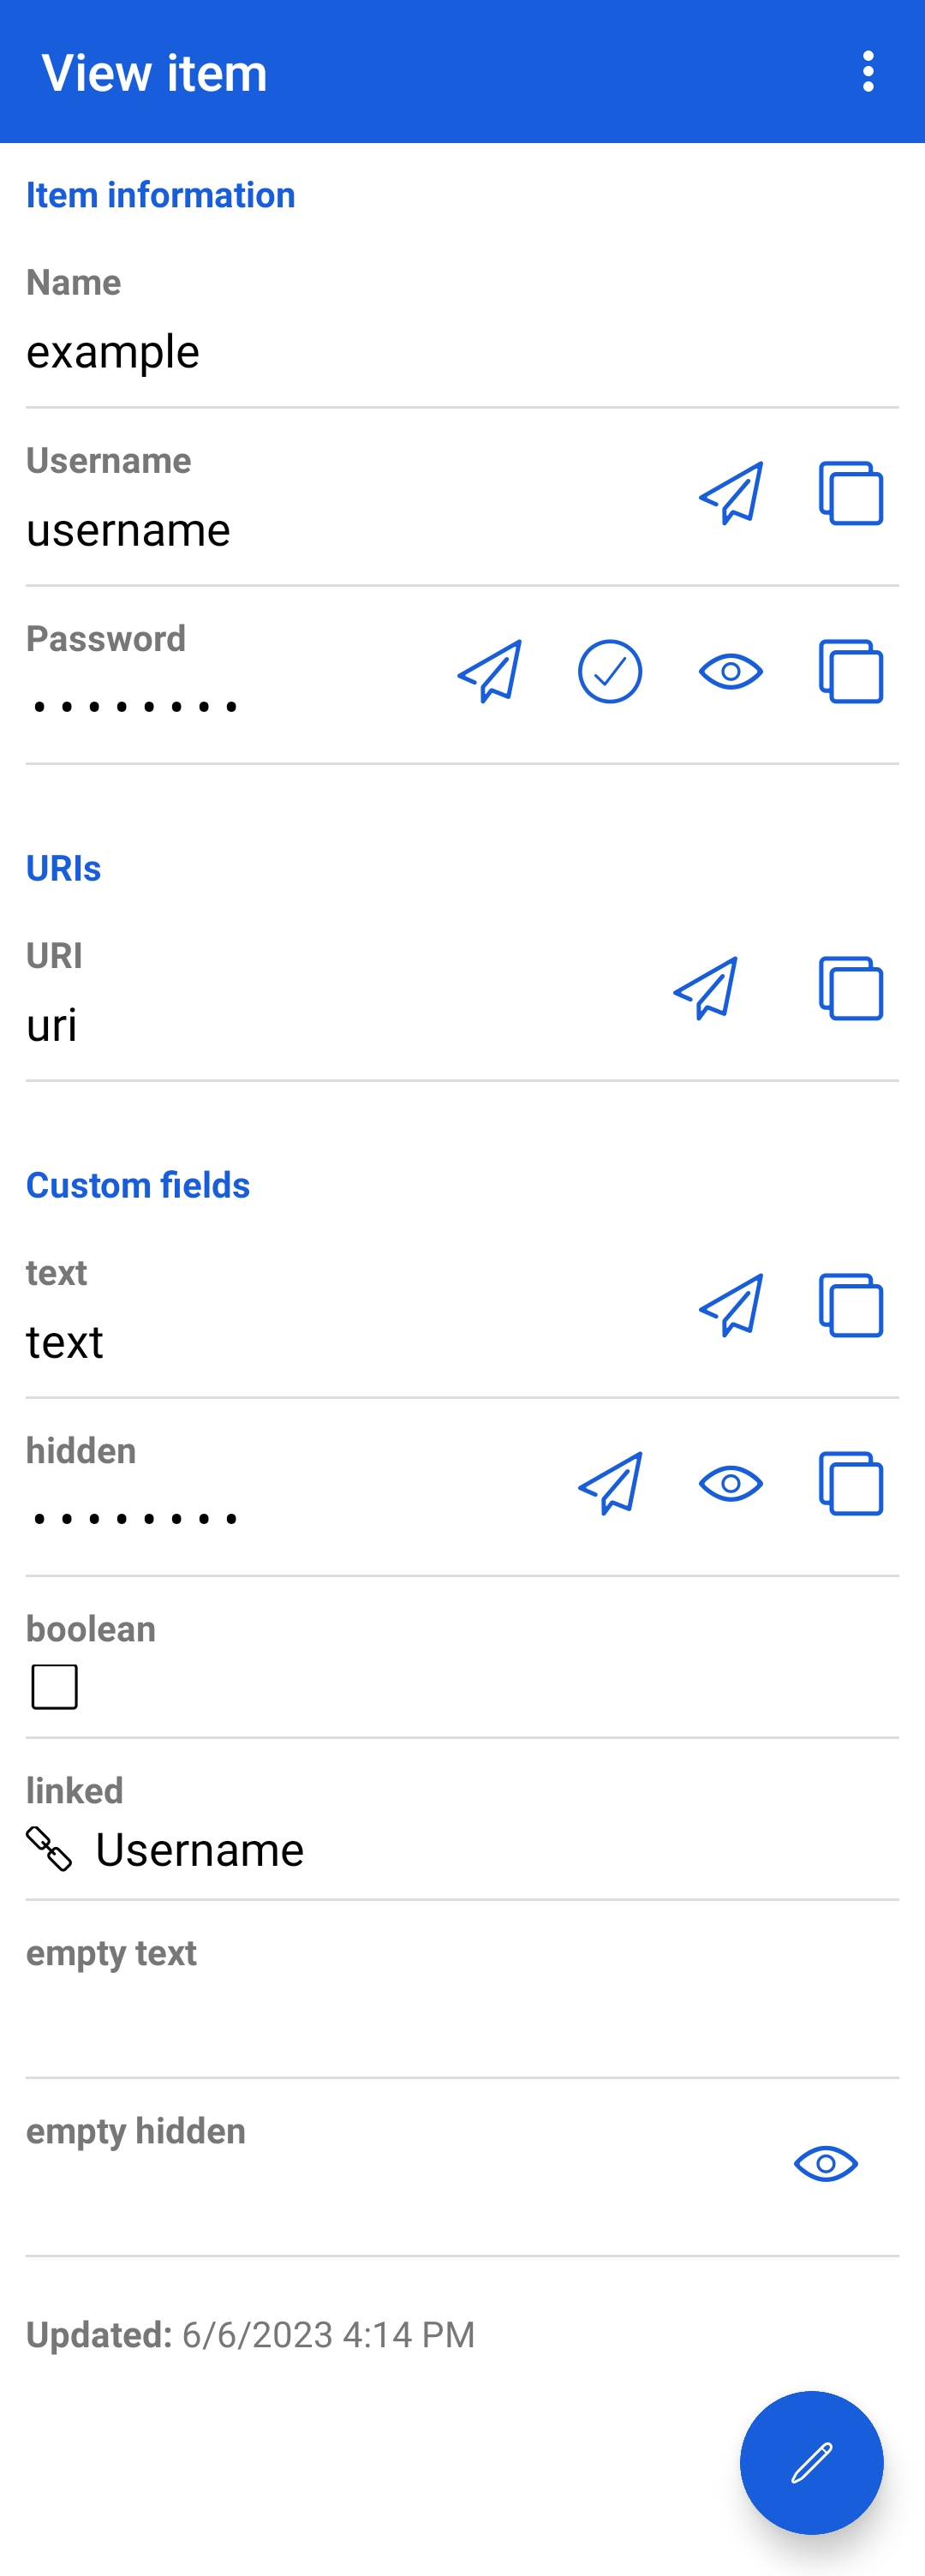
\includegraphics[width=0.4\columnwidth]{gfx/bitapp-mod-login.png}}
\caption{Pantalla de elemento. Modificación de la app de Bitwarden} % no se referencia \gls{login} porque hace que ocupe exactamente una línea más y por lo tanto pasa a la página siguiente
    \label{fig:bitapp-mod-login}
\end{figure}

\subsubsection{Repositorios}\label{repos}
Los cambios realizados se encuentran en el fork de GitHub de PabloOQ.
Debido a un problema de compatibilidad durante el desarrollo hubo que hacer un merge de la rama master de Bitwarden, todo el código se encuentra en:

\noindent\url{https://github.com/PabloOQ/mobile/tree/stick-after-merge}

\noindent Sin embargo, para visualizar rápidamente el código modificado antes de hacer el merge, se podría ver en esta rama (aunque este está también en la rama mencionada anteriormente):

\noindent\url{https://github.com/PabloOQ/mobile/tree/stick}

\noindent Finalmente en este enlace se muestra el código añadido, al ser el total no incluye el código previo a las refactorizaciones.

\noindent\url{https://github.com/PabloOQ/mobile/compare/tfg-diff...PabloOQ:mobile:stick-after-merge}

\noindent El informe escrito en LaTeX se encuentra en:

\noindent\url{https://github.com/PabloOQ/informeTFG}
\newpage

\subsubsection{Plan de trabajo}
En la tabla \ref{tab:plan_original} se muestra el plan de trabajo original.
\begin{table}[H]
\begin{tabular}{|p{0.25\textwidth}|p{0.12\textwidth}|p{0.48\textwidth}|}
\hline
Fases                                & Duración \newline Estimada & Tareas \\ \hline

Estudio previo / Análisis            & 85                & Tarea 1.1: Estudio de la aplicación de Bitwarden \newline Tarea 1.2: Estudio de la \gls{api} de InputStick \\ \hline

Diseño / Desarrollo / Implementación & 85                & Tarea 2.1: Diseño y creación de la interfaz de usuario \newline Tarea 2.2: Adaptar la \gls{api} de InputStick a C\# \newline Tarea 2.3: Implementación de InputStick a Bitwarden \\ \hline

Evaluación / Validación / Prueba     & 30                & Tarea 3.1: Verificación de la \gls{gui} \newline Tarea 3.2: Verificación de la funcionalidad nueva \\ \hline

Documentación / Presentación         & 100               & Tarea 4.1: Documentación de la \gls{gui} \newline Tarea 4.2: Documentación de la funcionalidad nueva \newline Tarea 4.3: Documentación de temas relacionados \\ \hline
\end{tabular}
\caption{Plan de trabajo original. Realización propia.}
\label{tab:plan_original}
\end{table}

Sin embargo realmente las horas dedicadas son las que se muestran en la tabla \ref{tab:plan_real}. Esto cambio se debe a que el estudio de la aplicación fue mucho más complejo de lo esperado y por tanto requirió mucho más tiempo.

\begin{table}[H]
\begin{tabular}{|p{0.25\textwidth}|p{0.12\textwidth}|p{0.48\textwidth}|}
\hline
Fases                                & Duración \newline Estimada & Tareas \\ \hline

Estudio previo / Análisis            & 115               & Tarea 1.1: Estudio de la aplicación de Bitwarden \newline Tarea 1.2: Estudio de la \gls{api} de InputStick \\ \hline

Diseño / Desarrollo / Implementación & 85               & Tarea 2.1: Diseño y creación de la interfaz de usuario \newline Tarea 2.2: Adaptar la \gls{api} de InputStick a C\# \newline Tarea 2.3: Implementación de InputStick a Bitwarden \\ \hline

Evaluación / Validación / Prueba     & 15                & Tarea 3.1: Verificación de la \gls{gui} \newline Tarea 3.2: Verificación de la funcionalidad nueva \\ \hline

Documentación / Presentación         & 85               & Tarea 4.1: Documentación de la \gls{gui} \newline Tarea 4.2: Documentación de la funcionalidad nueva \newline Tarea 4.3: Documentación de temas relacionados \\ \hline
\end{tabular}
\caption{Plan de trabajo real. Realización propia.}
\label{tab:plan_real}
\end{table}
\subsection{Pruebas con usuarios}
\subsubsection{Usuario de Bitwarden}
Se ha usado como usuario de prueba al mismo que originó la idea del proyecto. La opinión de dicho usuario es que es un poco complicado configurarlo, ya que no hay ningún aviso cuando la app InputStickUtility no está instalada, esto se suponía que debía ocurrir, si al intentar comunicarse con InputStickUtility esta no se encuentra instalada, \href{https://github.com/inputstick/InputStickAPI-Android/blob/81d9ce96aa9e4db4f508090f54bea981ffecfcb7/InputStickAPI/src/com/inputstick/api/broadcast/InputStickBroadcast.java\#L73}{la propia librería genera una ventana emergente}, sin embargo cuando dicho usuario lo probó, el diálogo no apareció, nuestra teoría es que está relacionado con \gls{jbl}, por lo que es algo a solucionar. El usuario plantea un tutorial de ventanas emergentes, lamentablemente esto es algo que estaría fuera de lugar en la app de Bitwarden, pues sería la única instancia donde encontrar dicho tutorial. El otro inconveniente que encontró era el hecho de tener en cuenta la distribución del teclado, pues es algo que realmente el usuario promedio no sabe que funciona así, y tampoco es fácil de comprender, lamentablemente es inevitable el tener que configurar la opción del teclado, y recae en el usuario, la única forma de solucionar esto sería explicándolo mejor. Creemos que actualmente este sistema innecesariamente complejo, y que su uso a día de hoy se debe simplemente a que es algo que se lleva usando mucho tiempo y cambiar a algo mejor sería una tarea en la que las compañías y grupos más grandes se tendrían que poner de acuerdo. Además de esto el usuario indicó que no se fijó en los nuevos botones porque asumía que la opción estaría en el menú desplegable, esto tiene fácil solución, indicándolo en la descripción de la configuración.

\subsubsection{Usuario de InputStick}
Lamentablemente, no es fácil encontrar a un usuario que conozca InputStick de antemano, así que se ha seleccionado un usuario y se le ha explicado el funcionamiento de InputStick. Tras ello y simplemente diciéndole el objetivo de la app de Bitwarden se le ha dejado navegar por la app modificada a ver si es capaz de desenvolverse. El único problema que encontró era activar la nueva funcionalidad, pues no sabía dónde descartó la configuración como pantalla para activar la funcionalidad, así que hemos intervenido, pero de resto no ha tenido mayor problema, con los textos en la pantalla de configuración lo ha comprendido fácilmente.
\subsection{Manual de usuario}
Para usar InputStick en Bitwarden el usuario deberá instalar la versión modificada de Bitwarden realizada en este proyecto, también deberá realizar la instalación de InputStickUtility. Una vez hecho esto, deberá iniciar sesión o registrarse en Bitwarden o Vaultwarden, así como configurar la clave de InputStick en InputStickUtility. Tras ello en los ajustes puede activar la funcionalidad y la configuración de la misma. Finalmente cuando quiera introducir los credenciales en otro dispositivo simplemente hay que conectar InputStick al dispositivo y acceder al \gls{login} ahí deberá pulsar en el icono de enviar, se le solicitará activar Bluetooth y el campo se escribirá automáticamente en donde se encuentre el foco en el dispositivo. En la figura \ref{fig:diagrama_de_usuario} vemos lo que ocurre a ojos del usuario.

\begin{figure}[H]
    \centering
    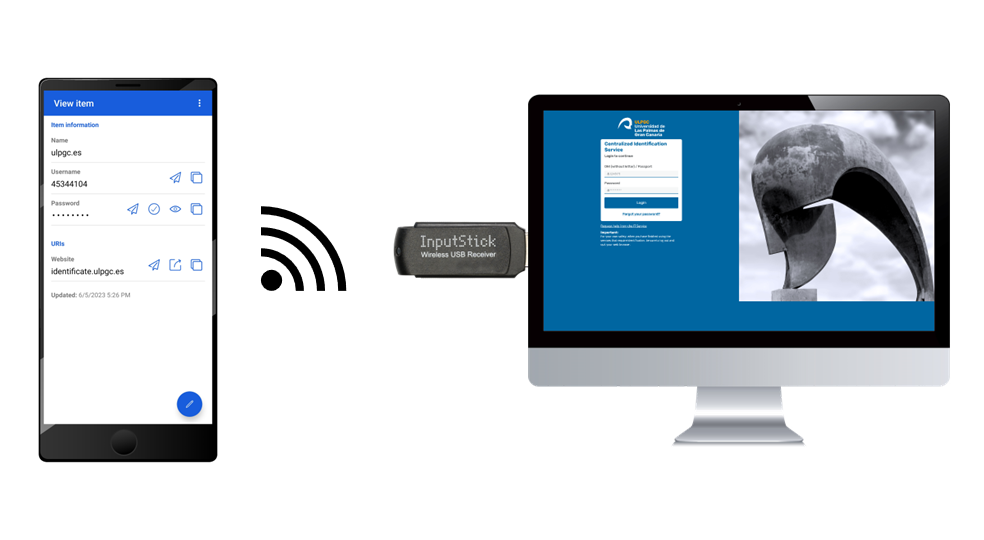
\includegraphics[width=\textwidth]{gfx/diagrama_de_usuario.png}
    \caption{Diagrama de usuario. Realización propia.}
    \label{fig:diagrama_de_usuario}
    El ordenador sobremesa es a modo de ejemplo, pero es sustituible por cualquier dispositivo compatible con \gls{usb} \gls{hid}.\newline
    Marco de móvil. Imagen por brgfx en Freepik.com.\newline
    Marco de monitor. Imagen por d3images en Freepik.com.\newline
\end{figure} \label{manual}
\subsection{Herramientas}
\begin{itemize}
    \item GitHub:
    Servidor git donde subir las versiones del proyecto.
    \item Sublime Merge:
    Cliente git para controlado de versiones.
    \item Visual Studio:
    Entorno de programación usado para el desarrollo de la aplicación, con extensión para desarrollo móvil en Xamarin.
    \item Obsidian:
    Editor de markdown para apuntar notas, con la extensión Kanban para la organización del proyecto, de esta forma es similar a otras herramientas como Trello, pero simplificado
    \item Overleaf:
    Editor de LaTeX online.
    \item Docker:
    Para hospedar la instancia de Vaultwarden se ha usado Docker, esta herramienta crea contenedores donde lanzar programas de forma compartimentada
    \item StarUML:
    Para el diagrama de casos de uso.
    \item Microsoft PowerPoint:
    Para el diagrama de conexiones.
\end{itemize}
\newpage

\section{Conclusión}
\subsection{Dificultades}
El mayor problema ha sido sin duda, entender el código de Bitwarden, sobre todo el patrón \gls{mvvm}, de hecho es algo normal en desarrolladores con no mucha experiencia\cite{García2023intro}, esto ha llevado mucho más tiempo del esperado, así como un tira y afloja constante con el código pues se ha tenido que refactorizar más veces de las necesarias por falta de comprensión en su funcionamiento. Antes de comenzar con el proyecto nuestras expectativas eran que la dificultad estuviese en usar la librería de InputStick, escrita en Java, en C\# y el uso de la librería de InputStick para la comunicación con el mismo. Sin embargo, Visual Studio se ocupa de añadir una capa intermedia para la compatibilidad con la capa, y el uso de InputStickBroadcast y InputStickUtility facilita mucho el uso de la librería. La \gls{api} de InputStick se puede usar de forma más profunda pero perdiendo las comodidades aportadas por InputStickUtility, esto era el objetivo del proyecto, sin embargo se usó la parte \quotes{simple} de la librería a modo de plantilla y a medida que el proyecto avanzaba quedaba cada vez más claro que no iba a dar tiempo de cambiarlo.
\subsection{Reflexión}
Este proyecto me ha permitido entender mucho mejor el uso de ciertos patrones arquitectónicos, además de indagar en el ámbito de la criptografía que no se entraba en tanta profundidad en la rama que he cursado. Así como aprender a usar LaTeX. También me he familiarizado con C\#, lenguaje en el que no había escrito nunca. También he aprendido a estimar mejor el tiempo de trabajo, como se muestra en las tablas \ref{tab:plan_original} y \ref{tab:plan_real}, el tiempo dedicado no fue el esperado.
\newpage
\subsection{Futuro del proyecto}
Debido a que la estimación del tiempo del proyecto no fue correcta, algunas ideas se han quedado en el tintero, estas son mejoras que se podrían realizar
\begin{itemize}
    \item Eliminar InputStickUtility como intermediario:

Al usar InputStickBroadcast, es necesario tener instalada la app InputStickUtility. Con un uso más profundo de la librería de InputStick se puede eliminar esta limitación.

    \item Conexión directa por Bluetooth, sin InputStick como intermediario:
    
Esto eliminaría InputStick en casos donde tenga sentido. Por ejemplo, este proyecto se planteó al querer iniciar sesión en un dispositivo en el que no se confiaba, pero no como única opción. Si alguien quisiese hacer uso de esta funcionalidad con frecuencia en su hogar, por ejemplo en una consola de videojuegos y en una \textit{Smart TV}, que no son capaces de instalar un cliente de Bitwarden. En esta situación resultaría molesto tener que cambiar InputStick con frecuencia entre estos dispositivos, que suelen estar en un mueble o pegados a la pared, y por tanto con acceso incómodo a sus puertos. Sin embargo este tipo de dispositivos con mucha frecuencia tienen la posibilidad de conectar mandos de control mediante Bluetooth. Habría además que seguir teniendo en cuenta el protocolo \gls{hid} pues Bluetooth usa exactamente la misma definición que en \gls{usb}\cite{bluetoothhid}. La base hecha en este proyecto facilitaría esto, y esta nueva funcionalidad complementaría la anterior, en el hogar con dispositivos conocidos y compatibles se podría usar Bluetooth, en el exterior y en dispositivos no compatibles se podría usar InputStick.\newline

    \item Facilitar la identificación de la disposición del tecla:

Algunos dispositivos no permiten configurar la disposición, lo que resulta en un desconocimiento total de cuál es la disposición que está usando el dispositivo. Un sistema de ayuda para encontrar la disposición podría solventar este problema. Se podría enviar un texto de prueba al dispositivo, en el móvil se muestra  y el usuario introduce en el móvil los caracteres que faltan o distintos, entonces el móvil muestra diferentes opciones de lo que puede haber aparecido en su lugar en el dispositivo, luego el usuario selecciona entre las distintas opciones y el móvil informa al usuario de la disposición que está usando el dispositivo. En la figura \ref{fig:diagrama_texto} se muestra una maqueta. Si un carácter fuese incorrecto el usuario lo podría introducir en el cuadrado situado debajo de dicho carácter. Tampoco es necesario hacer una muestra tan grande, realizando un estudio se podría comprobar qué posiciones tienen tendencia a cambiar entre disposiciones y así minimizar el texto escrito, para no abrumar al usuario.

\begin{figure}[H]
    \centering
    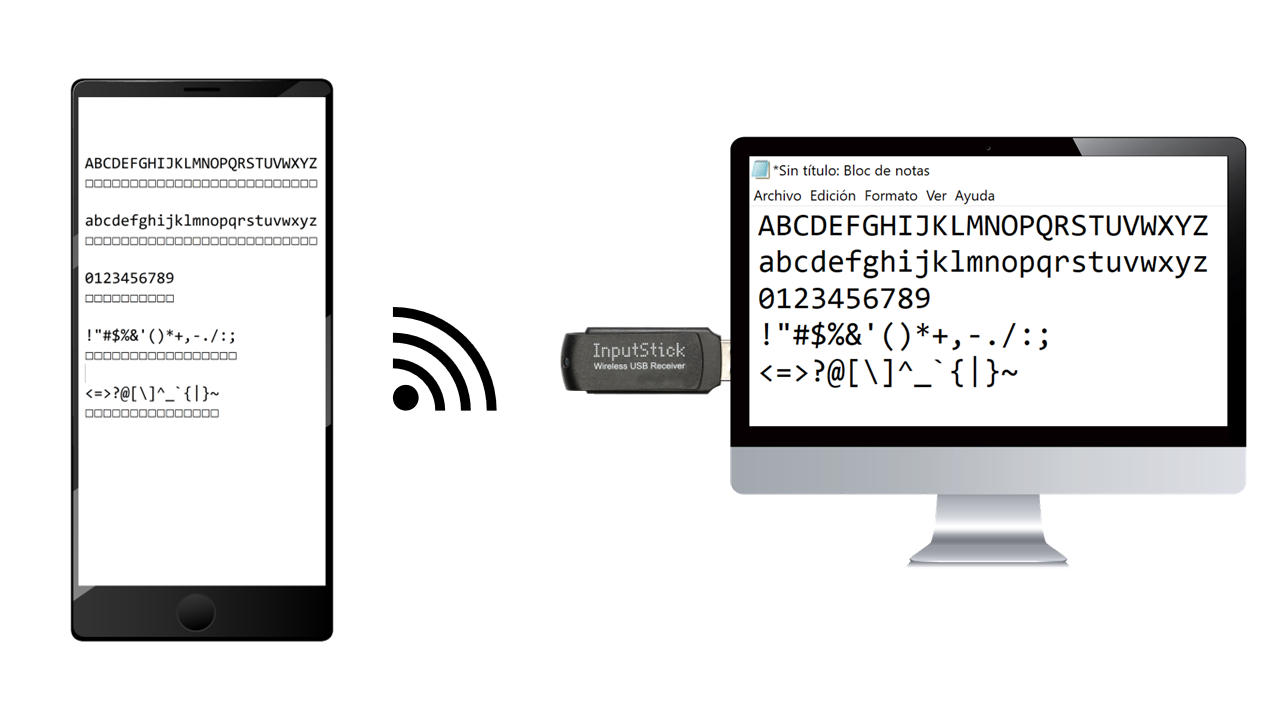
\includegraphics[width=\textwidth]{gfx/diagrama_texto.png}
    \caption{Maqueta de identificación de disposición. Realización propia.}
    \label{fig:diagrama_texto}
    El ordenador sobremesa es a modo de ejemplo, pero es sustituible por cualquier dispositivo compatible con \gls{usb} \gls{hid}.\newline
    Marco de móvil. Imagen por brgfx en Freepik.com.\newline
    Marco de monitor. Imagen por d3images en Freepik.com.\newline
\end{figure}

\end{itemize}
\newpage

\section{Licencias}
Este TFT usa códigos Open Source de diversas fuentes, así pues en esta sección se cumple el contrato puesto por estas licencias.
\subsection{Bitwarden mobile}
Bitwarden mobile  usa la licencia GPL 3.0. Como el objetivo principal de este proyecto es la modificación de este código, los cambios realizados se encuentran en el fork de GitHub de PabloOQ.
Debido a un problema de compatibilidad durante el desarrollo hubo que hacer un merge de la rama master de Bitwarden, todo el código se encuentra en:

\noindent\url{https://github.com/PabloOQ/mobile/tree/stick-after-merge}

\noindent Sin embargo, para visualizar rápidamente el código modificado antes de hacer el merge, se podría ver en esta rama (aunque este está también en la rama mencionada anteriormente):

\noindent\url{https://github.com/PabloOQ/mobile/tree/stick}

\subsection{Vaultwarden}
Vaultwarden usa la licencia GPL 3.0. Este código no ha sido modificado, simplemente se ha usado para crear una estancia vaultwarden en la que hacer pruebas de la aplicación de Bitwarden para Android.

\subsection{InputStick}
En GitHub la API de InputStick no tiene la licencia establecida, por ello se le preguntó personalmente al creador y él dió el visto bueno, sin poner ningún tipo de condición.

\subsection{GNU GPL 3}
\url{https://www.gnu.org/licenses/gpl-3.0.en.html}

% https://www.freepik.com/free-vector/blank-smartphone-icon-isolated-white-background_9688880.htm#query=phone&position=0&from_view=author
% https://www.freepik.com/free-vector/computer-design_919225.htm#query=monitor%20screen&position=1&from_view=search&track=ais
% https://www.freepik.com/free-vector/two-black-server-racks-realistic-illustration_3907757.htm
\newpage

% FIXME debería salir la bibliografía en el índice?
\bibliographystyle{IEEEtran}
\bibliography{bibliografia}

\end{document}

